\chapter{Experiments} \label{chap:exp}

In order to evaluate our proposed algorithms, the heuristic balancing method (\emph{GM}), the distance based node clustering scheme (\emph{DIST}), as well as the combination of those (\emph{HDM}), we compare them with the geometric monitoring method~\cite{Sharfman2006GM} (\emph{GM}), and the hierarchical clustering method of~\cite{Keren2014GMHetStreams} (\emph{DISTR}). Datasets originate from both synthetic and real-world settings in order to explore the performance, scalability and applicability of our methods in terms of reduction in communication.

Firstly, Section~\ref{sec:datasets} contains a detailed description of the datasets and the monitoring functions used for evaluation purposes. Following that, Section~\ref{sec:exp} presents the experimental results along with the necessary commentation.

\section{Data, Setup and Monitoring Functions} \label{sec:datasets}

\subsection{Synthetic Datasets}

Synthetic datasets have been incorporated into the evaluation process of the proposed algorithms in order to provide a controllable environment under which the behavior of our methods can be analyzed. Data streams are created by firstly sampling data stream velocity distribution means by a user specified normal distribution and fixing the standard deviation of each stream. Afterwards, an initial velocity is sampled from each stream's assigned distribution and a $\lambda$ value is chosen, which controls the rate of change of the streams' velocity. Stream update $v_i(t_k)$ of node $n_i$ at time $t_k$ is generated by sampling a new velocity $u_{k+1}$ from the velocity distribution assigned to node $n_i$ and updating the streams' value by: $v_i(t_{k+1})=v_i(t_k) + (1-\lambda)u_{k} + \lambda u_{k+1}$. Noisy versions of the generated streams are the product of additive Gaussian noise.

Linear streams (\emph{LIN}) are generated by setting the parent distribution to $\mathcal{N}(10,20)$, the standard deviation of each stream's velocity distribution to $\sigma=10$ and the lambda value to $\lambda=0$. An example of the resulting one dimensional streams corresponding to 20 nodes, along with the resulting global statistics stream, is illustrated in Figure~\ref{fig:linearStreams}.

Interweaving streams(\emph{INT}) are produced from the same parent distribution $\mathcal{N}(10,20)$ by selecting $\sigma=50$ for the standard deviation of each stream's velocity distribution and $\lambda=0.1$ as the velocity update parameter. An instance of one dimensional interweaving streams corresponding to 20 nodes, along with the resulting global statistics stream, is shown in Figure~\ref{fig:intStreams}.

Noisy streams (\emph{NOISE}) are the result of the previously used parent distribution with $\sigma=100$ as the standard deviation of each stream's velocity, $\lambda=0.15$ the velocity update parameter, and  $\mathcal{N}(0,30)$ the distribution of the additive Gaussian noise. Such one dimensional streams corresponding to 20 monitoring nodes, along with the resulting global statistics stream, are depicted in Figure~\ref{fig:noiseStreams}.

When necessary, a partitioning of the dataset into training and testing sets is executed by uniformly sampling $20\%$ of the initial dataset as the training set, with the rest being the testing dataset. 

Unless stated otherwise, thresholds are set to $1*10^4$ for the \emph{LIN} dataset, $2*10^3$ for the \emph{INT} dataset, and $2.5*10^3$ for the \emph{NOISE} dataset, irrespective of the number of streams in each experiment. 

%%%%%%%%%%%%%%%%%%%%%%%%%%%%%%%%%LIN synthetic datasets figure %%%%%%%%%%%%%%%%%%%%%%%%%%%%
\begin{figure*}[!h]
\centering
\begin{subfigure}[t]{0.49\textwidth}
\centering
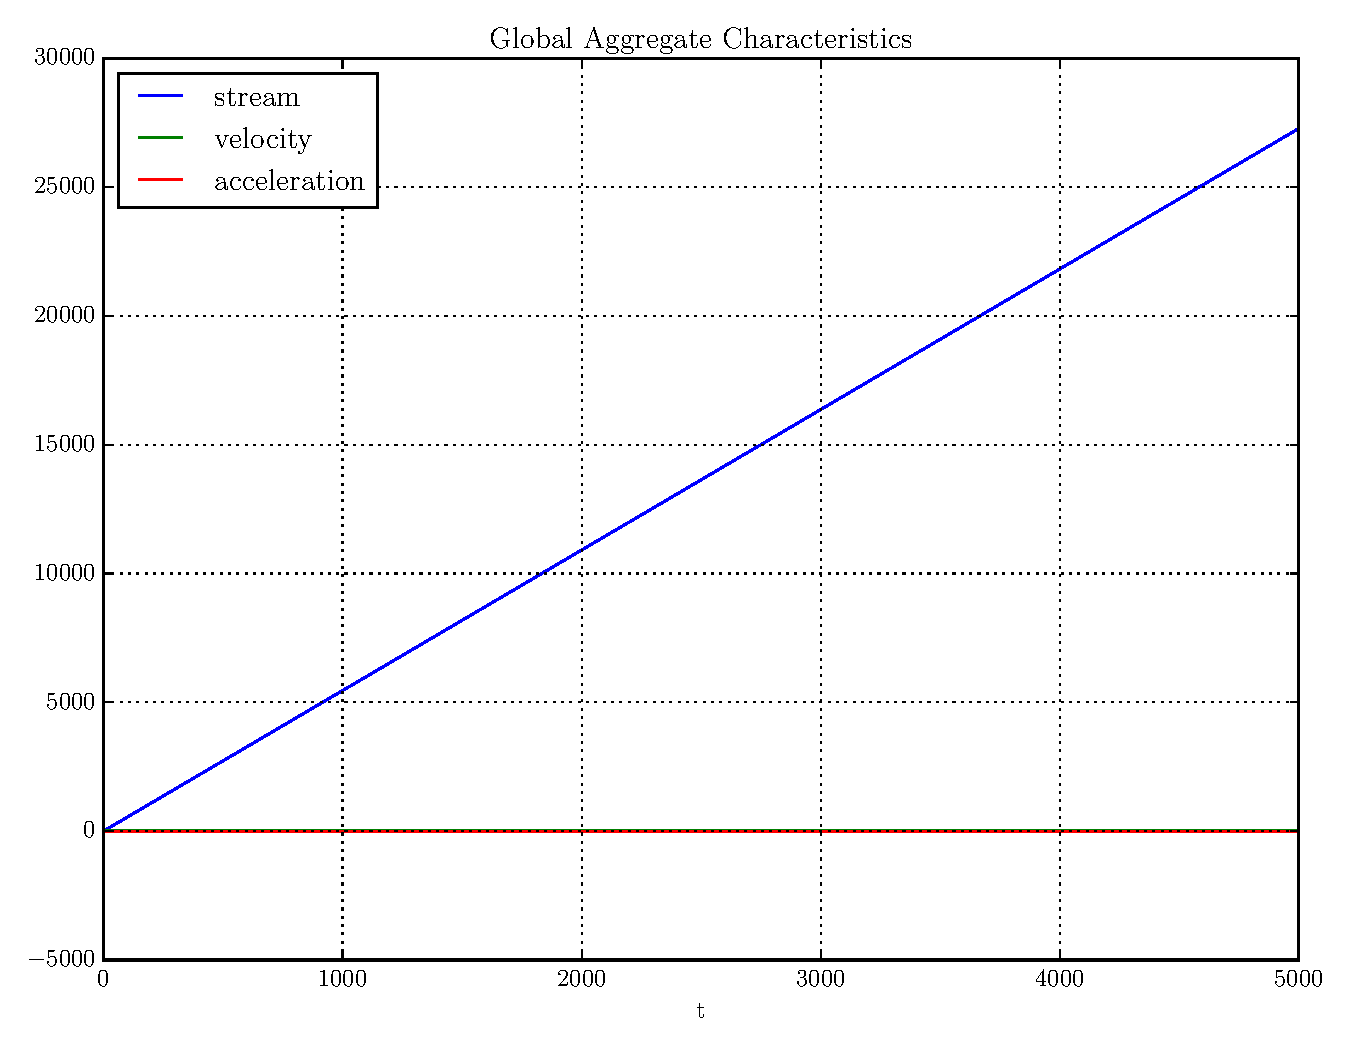
\includegraphics[scale=0.36, trim=2cm 0 0 0]{img/linear1D20N_global.pdf}
\caption{LIN global statistics stream of 20 streams}
\end{subfigure}
\begin{subfigure}[t]{0.49\textwidth}
\centering
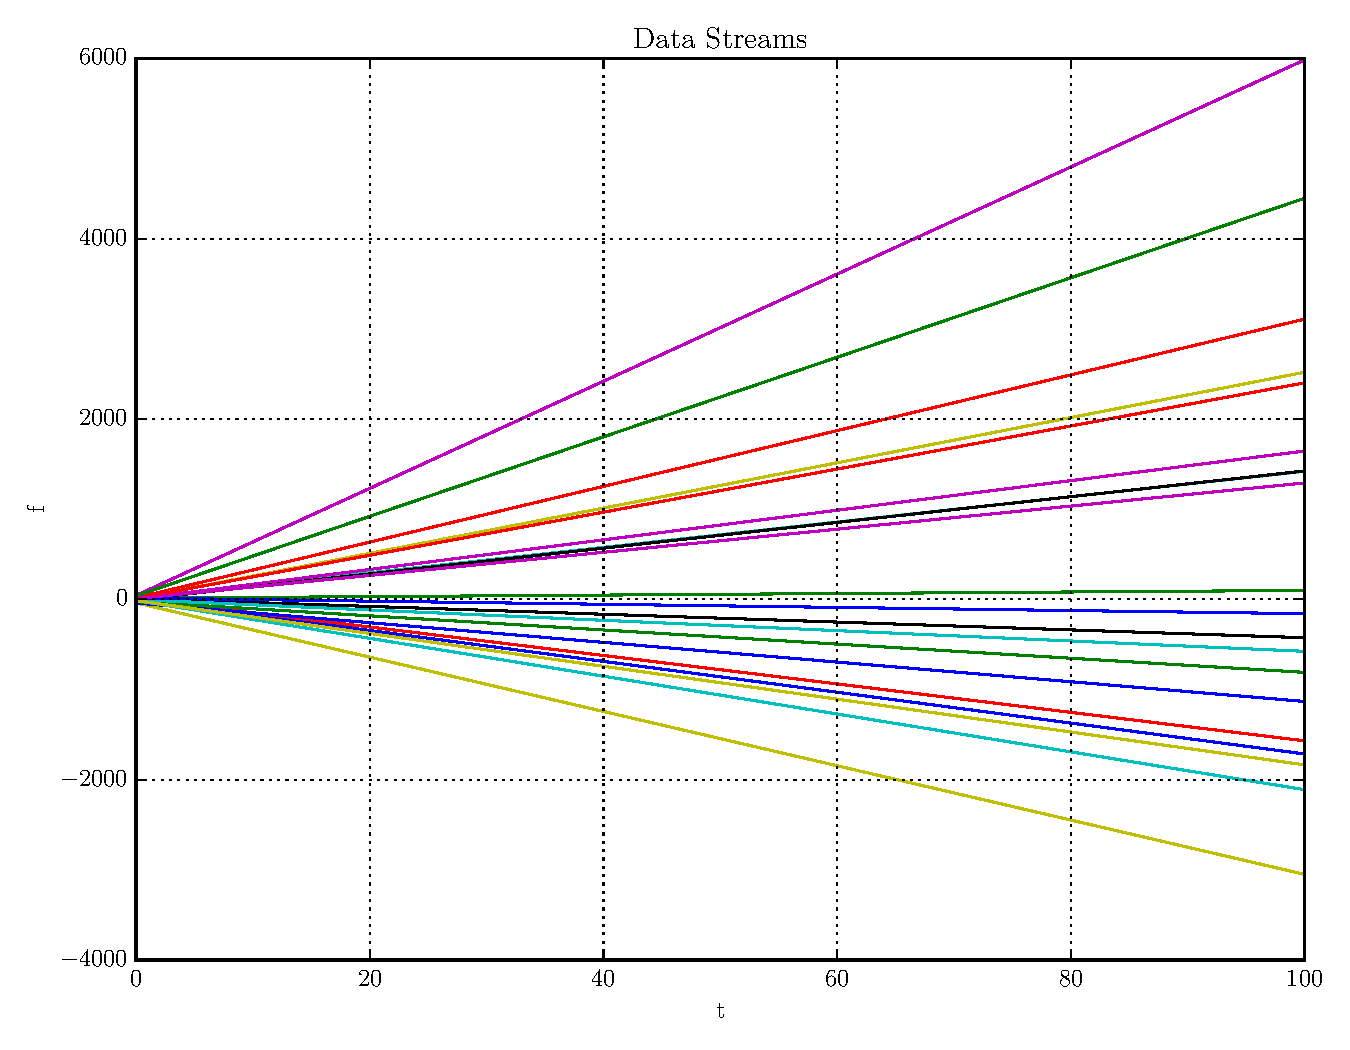
\includegraphics[scale=0.36]{img/linear1D20N_streams.pdf}
\caption{LIN local statistics streams of 20 nodes} 
\end{subfigure}
\vspace{0.5cm}
\caption{Linear data stream examples (LIN)}\label{fig:linearStreams}
\end{figure*}
%%%%%%%%%%%%%%%%%%%%%%%%%%%%%%%%%%%%%%%%%%%%%%%%%%%%%%%%%%%%%%%%%%%%%%%%%%%%%%%%%%%%%%%%%%%

%%%%%%%%%%%%%%%%%%%%%%%%%%%%%%%%%INT synthetic datasets figure %%%%%%%%%%%%%%%%%%%%%%%%%%%%
\begin{figure*}[!h]
\centering
\begin{subfigure}[t]{0.49\textwidth}
\centering
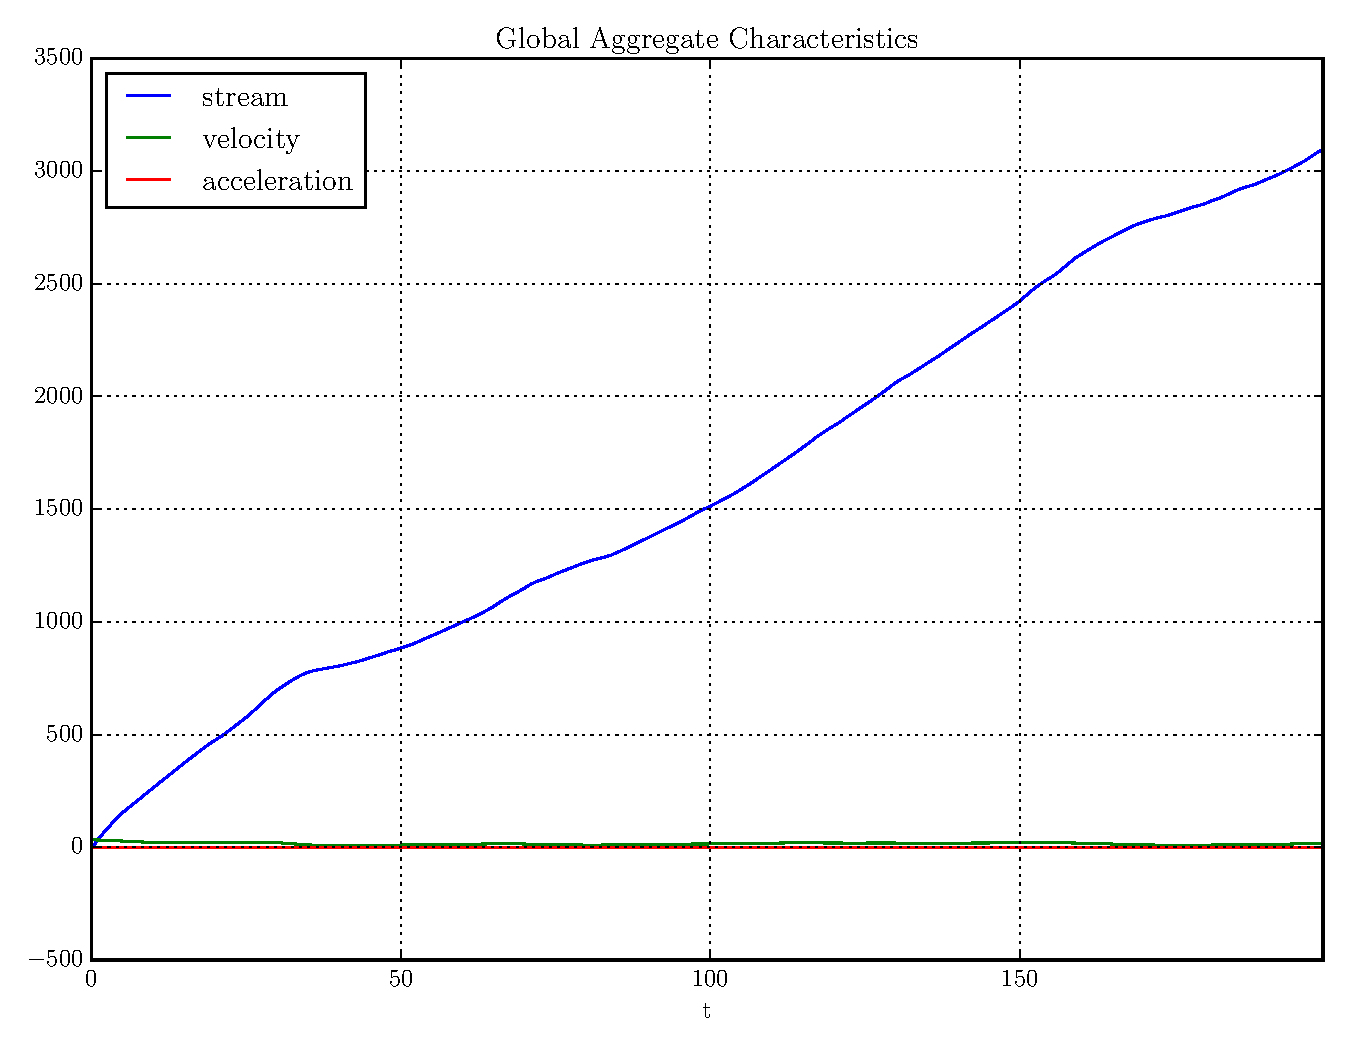
\includegraphics[scale=0.36, trim=2cm 0 0 0]{img/interweaving1D20N_global.pdf}
\caption{INT global statistics stream of 20 streams}
\end{subfigure}
\begin{subfigure}[t]{0.49\textwidth}
\centering
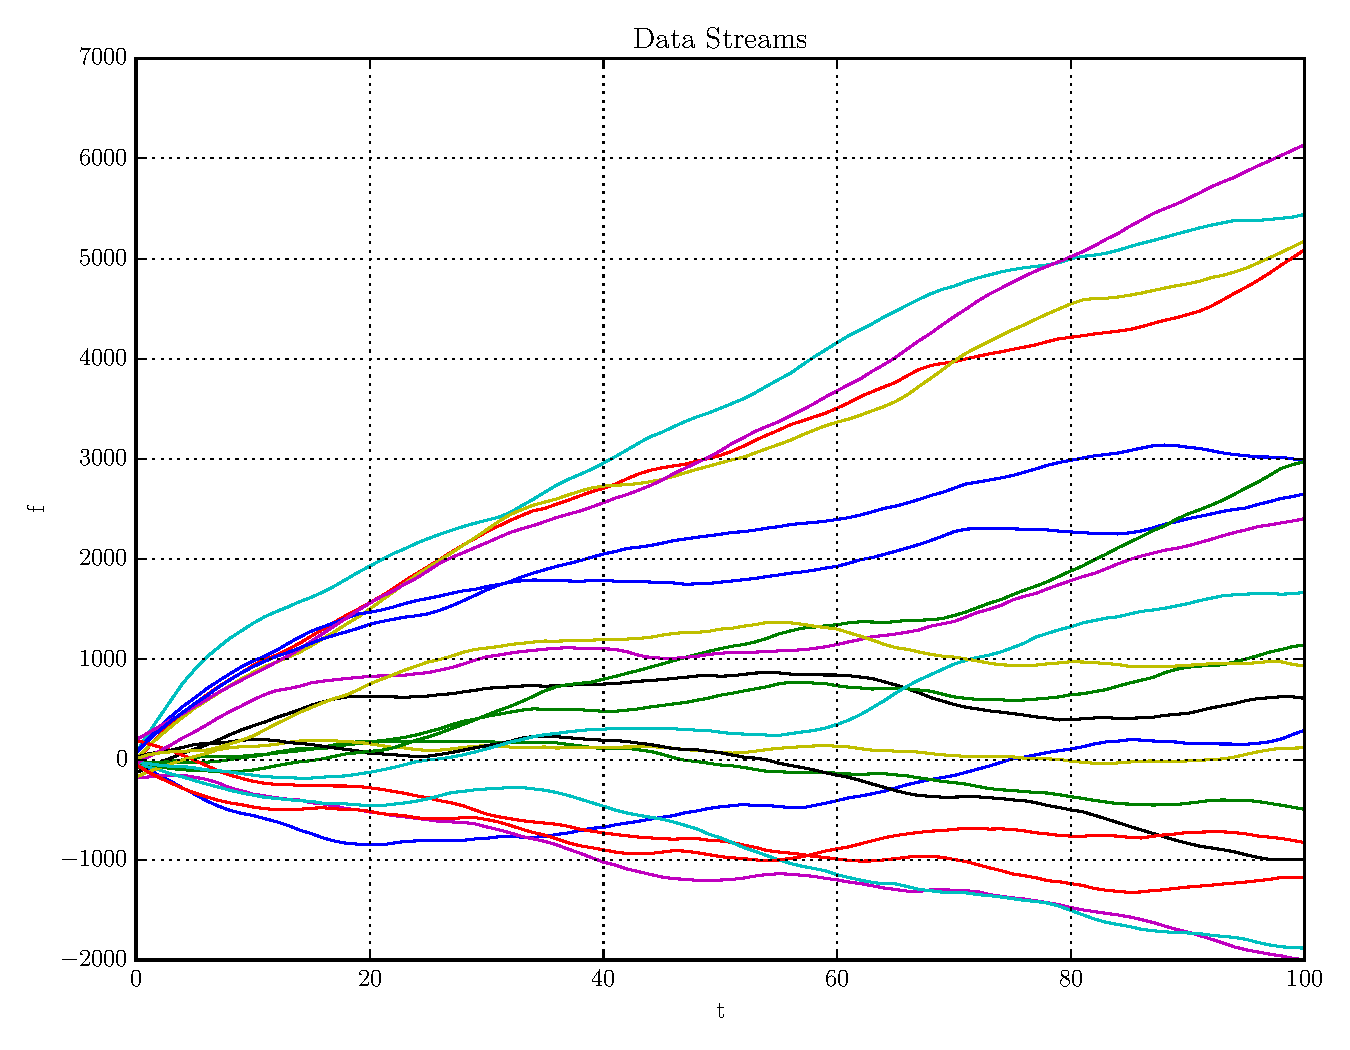
\includegraphics[scale=0.36]{img/interweaving1D20N_streams.pdf}
\caption{INT local statistics streams of 20 nodes} 
\end{subfigure}
\vspace{0.5cm}
\caption{Interweaving data stream examples (INT)}\label{fig:intStreams}
\end{figure*}
%%%%%%%%%%%%%%%%%%%%%%%%%%%%%%%%%%%%%%%%%%%%%%%%%%%%%%%%%%%%%%%%%%%%%%%%%%%%%%%%%%%%%%%%%%%

%%%%%%%%%%%%%%%%%%%%%%%%%%%%%%%%NOISE synthetic datasets figure %%%%%%%%%%%%%%%%%%%%%%%%%%%%
\begin{figure*}[!h]
\centering
\begin{subfigure}[t]{0.49\textwidth}
\centering
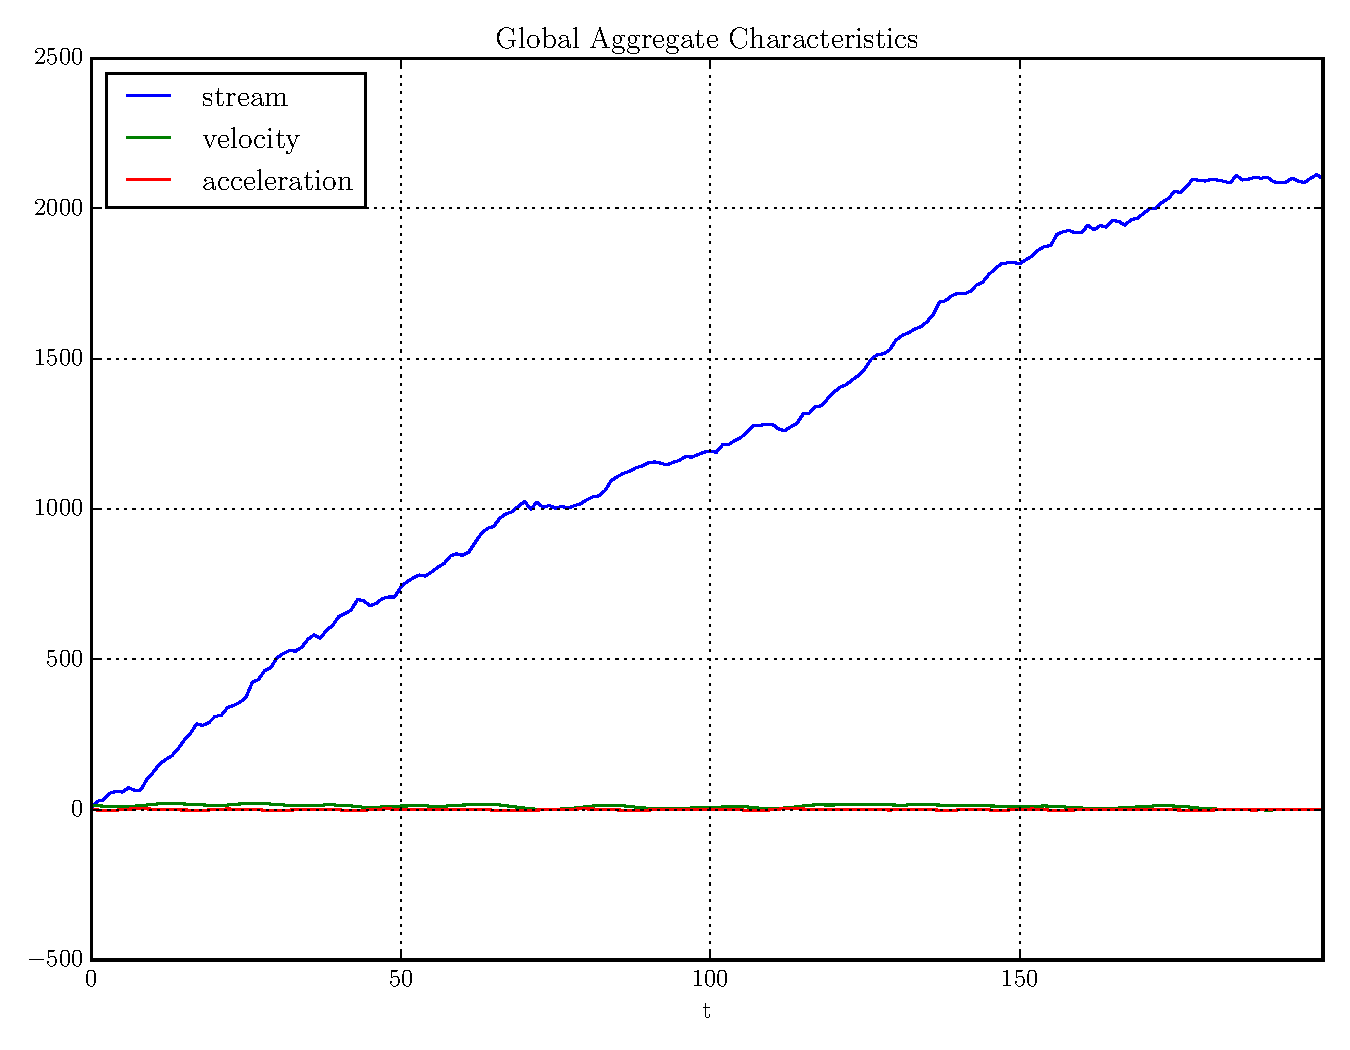
\includegraphics[scale=0.36, trim=2cm 0 0 0]{img/noisyinterweaving1D20N_global.pdf}
\caption{NOISE global statistics stream of 20 streams}
\end{subfigure}
\begin{subfigure}[t]{0.49\textwidth}
\centering
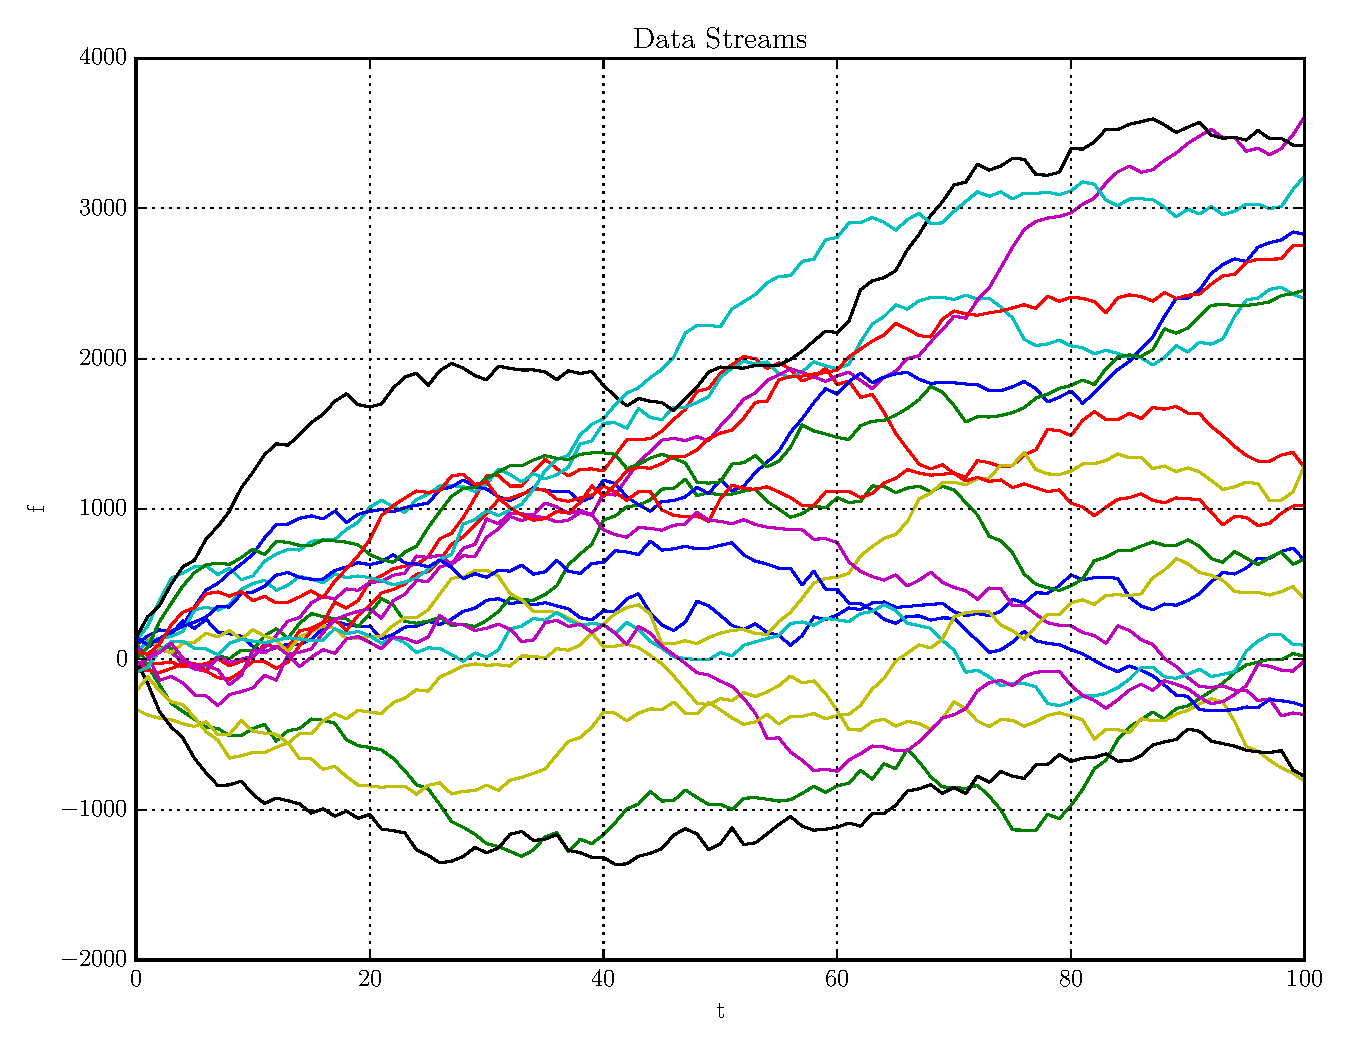
\includegraphics[scale=0.36]{img/noisyinterweaving1D20N_streams.pdf}
\caption{NOISE local statistics streams of 20 nodes} 
\end{subfigure}
\vspace{0.5cm}
\caption{Interweaving data stream examples (NOISE)}\label{fig:noiseStreams}
\end{figure*}
%%%%%%%%%%%%%%%%%%%%%%%%%%%%%%%%%%%%%%%%%%%%%%%%%%%%%%%%%%%%%%%%%%%%%%%%%%%%%%%%%%%%%%%%%%%
%TODO: include actual dataset?
\subsection{Air Quality Database}
%%%%%%%%%%%%%%%%%%%%%%%%%%%%%%%%NO2_NO actual datasets figure %%%%%%%%%%%%%%%%%%%%%%%%%%%%%
\begin{figure*}[!h]
\centering
\begin{subfigure}[t]{0.49\textwidth}
\centering
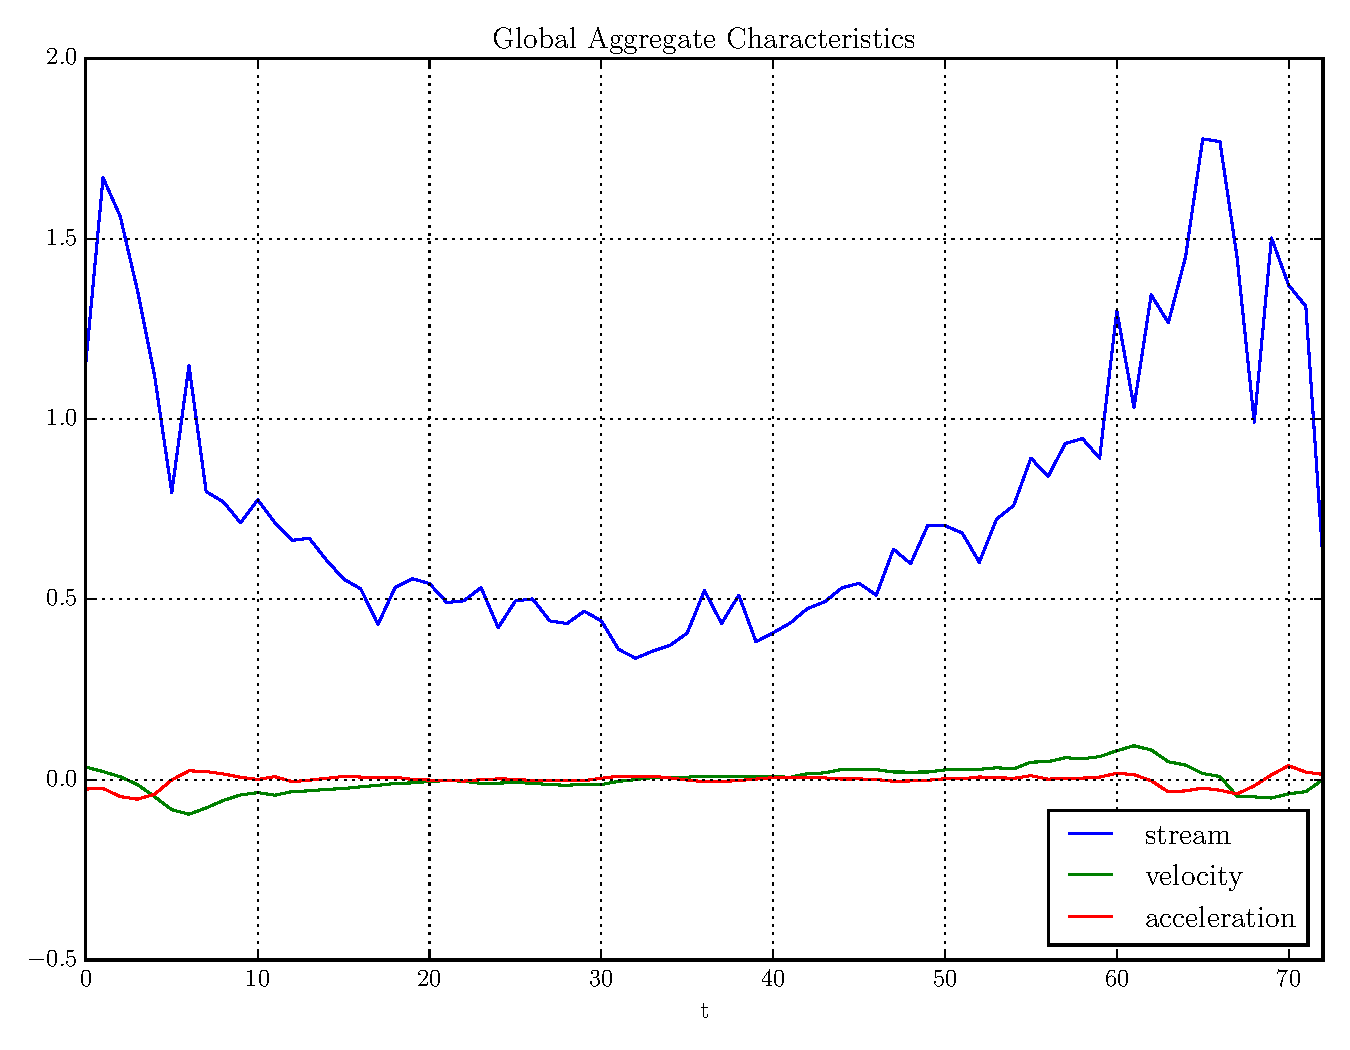
\includegraphics[scale=0.34, trim=2cm 0 0 0]{img/AT_NO2_NO_2014_8N_global.pdf}
\caption{Global statistics stream of 8 nodes monitoring the ratio $NO/NO_2$.}
\end{subfigure}
\begin{subfigure}[t]{0.49\textwidth}
\centering
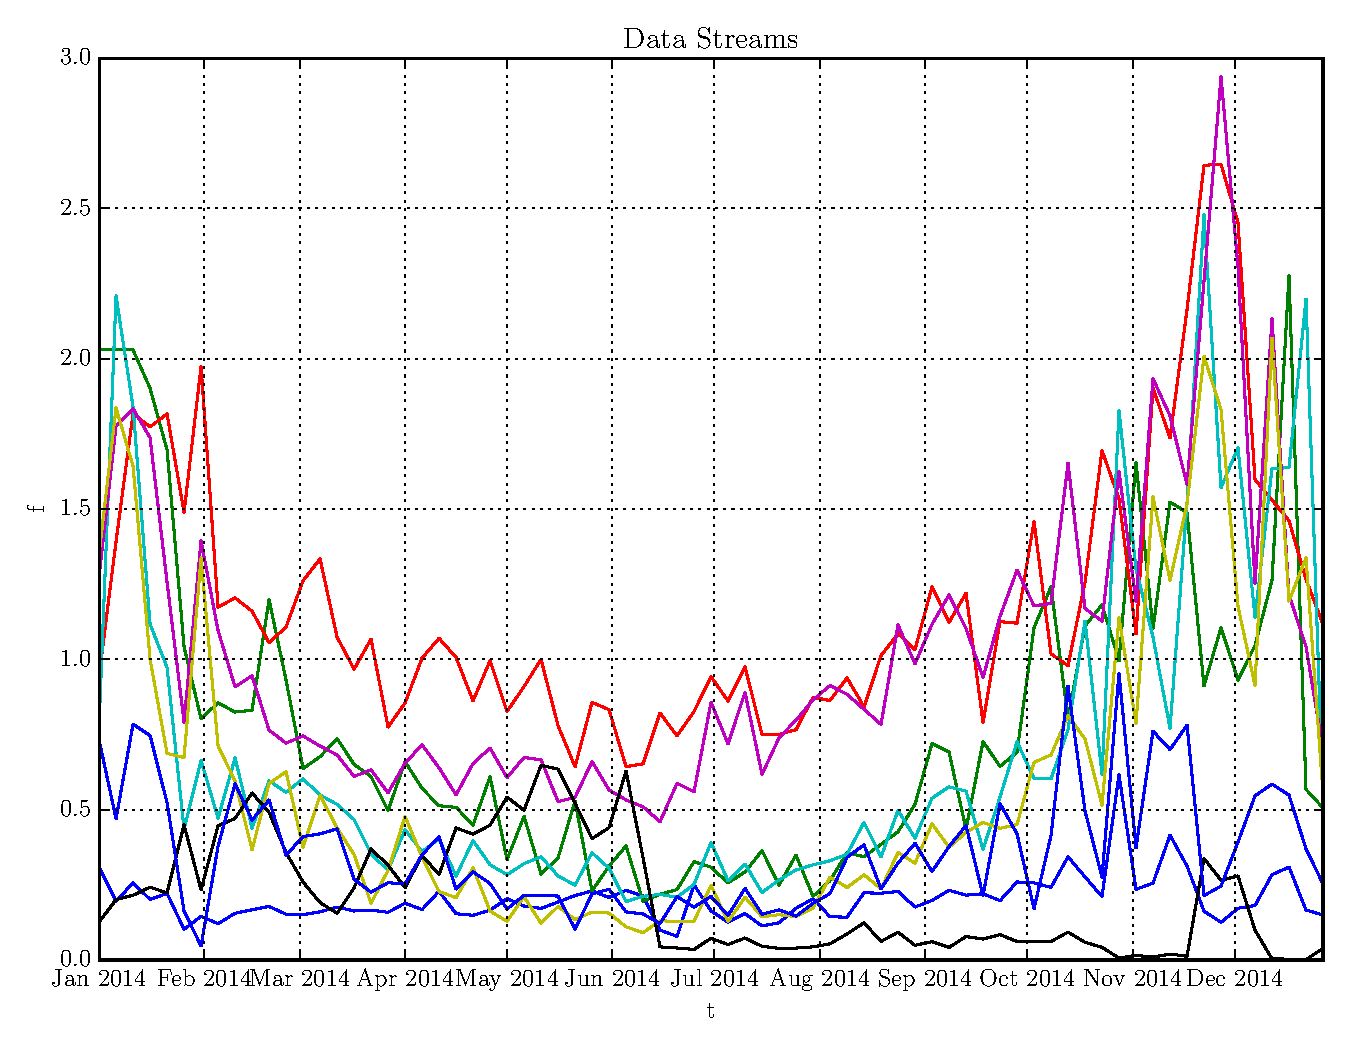
\includegraphics[scale=0.34]{img/AT_NO2_NO_2014_8N_streams.pdf}
\caption{Local statistics streams of 8 nodes monitoring the ratio $NO/NO_2$.} 
\end{subfigure}
\vspace{0.5cm}
\caption{Streams of 8 nodes monitoring the ratio $NO/NO_2$.}\label{fig:NO2_NO}
\end{figure*}
%%%%%%%%%%%%%%%%%%%%%%%%%%%%%%%%%%%%%%%%%%%%%%%%%%%%%%%%%%%%%%%%%%%%%%%%%%%%%%%%%%%%%%%%%%%
%%%%%%%%%%%%%%%%%%%%%%%%%%%%%%%%NO2_sq actual datasets figure %%%%%%%%%%%%%%%%%%%%%%%%%%%%
\begin{figure*}[!h]
\centering
\begin{subfigure}[t]{0.49\textwidth}
\centering
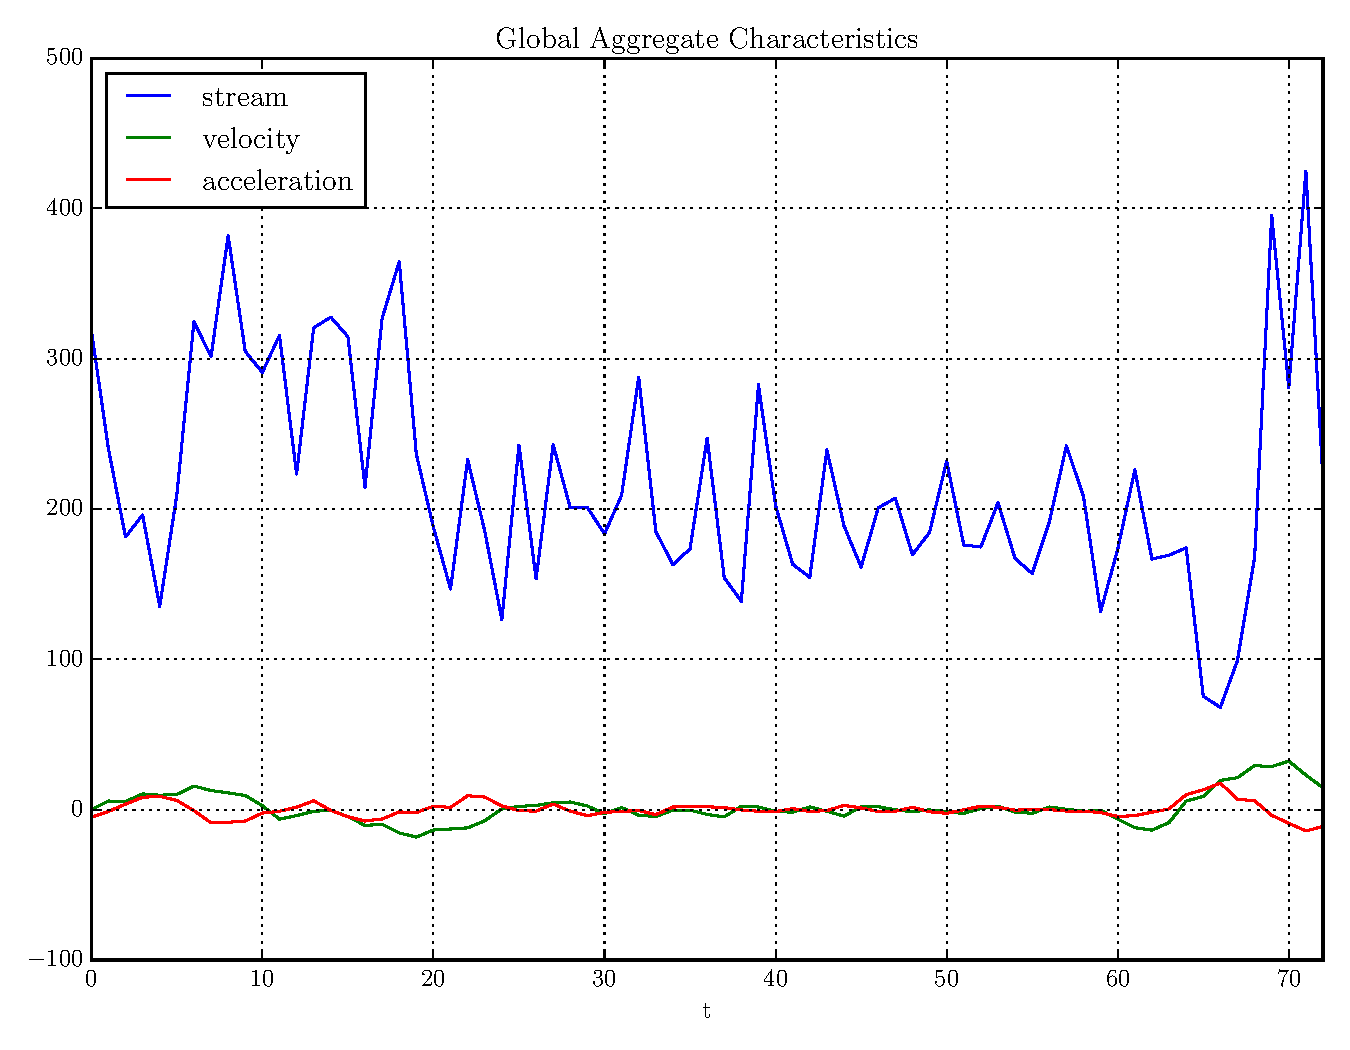
\includegraphics[scale=0.34, trim=2cm 0 0 0]{img/AT_NO2_sq_2014_8N_global.pdf}
\caption{Global statistics stream of 8 nodes monitoring the variance of $NO_2$ air pollutant.}
\end{subfigure}
\begin{subfigure}[t]{0.49\textwidth}
\centering
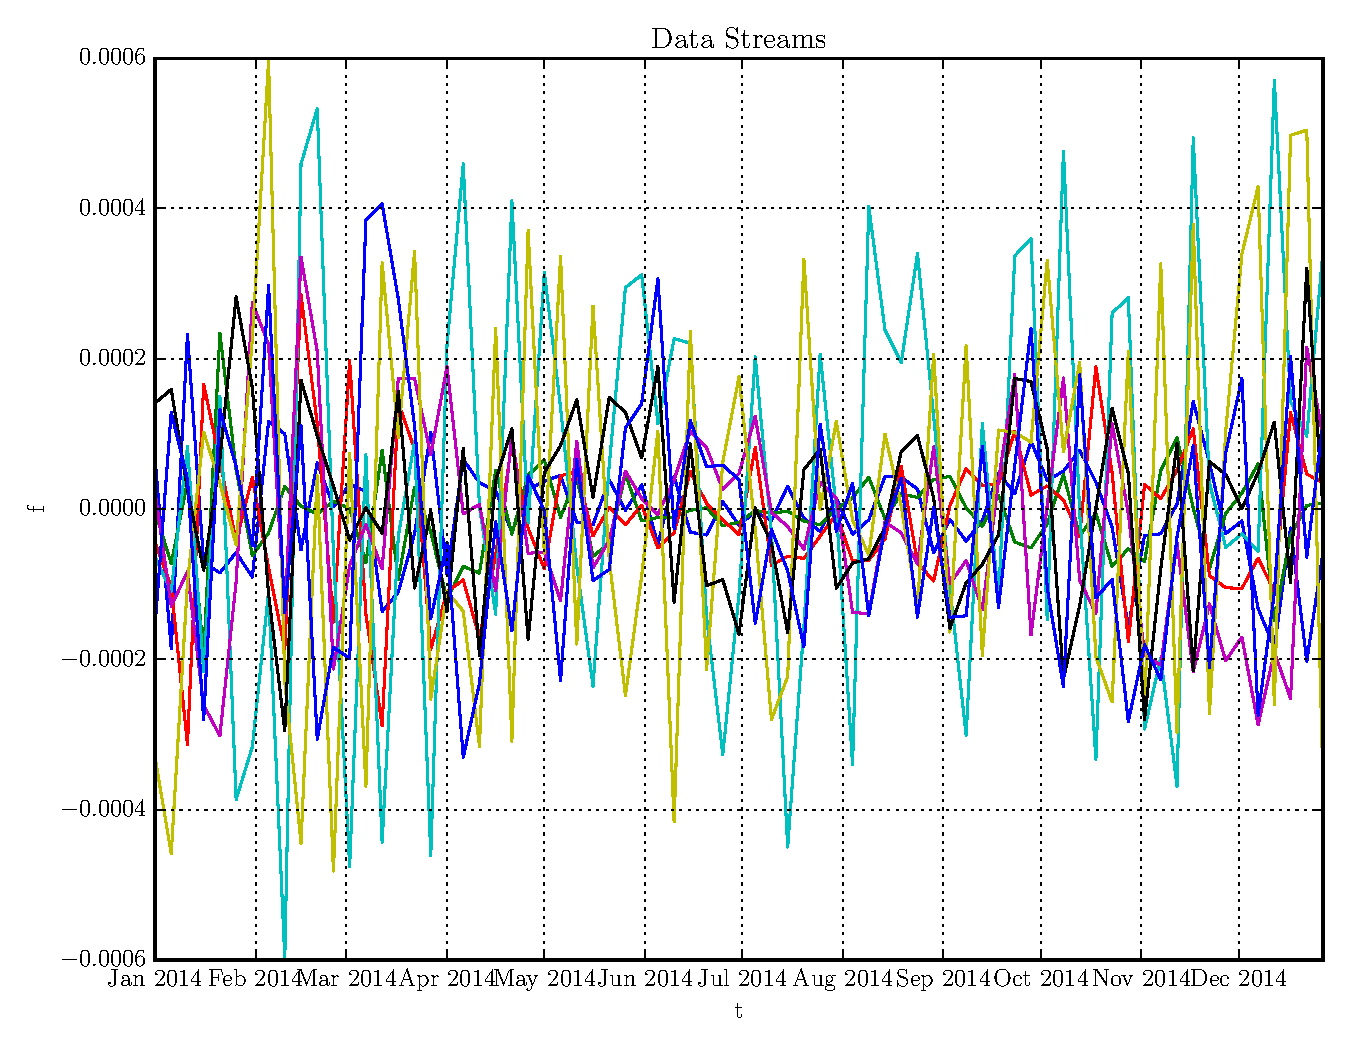
\includegraphics[scale=0.34]{img/AT_NO2_sq_2014_8N_streams.pdf}
\caption{Local statistics streams of 8 nodes monitoring the variance of $NO_2$ air pollutant.} 
\end{subfigure}
\vspace{0.5cm}
\caption{Streams of 8 nodes monitoring the variance of $NO_2$ air pollutant.}\label{fig:NO2_sq}
\end{figure*}
%%%%%%%%%%%%%%%%%%%%%%%%%%%%%%%%%%%%%%%%%%%%%%%%%%%%%%%%%%%%%%%%%%%%%%%%%%%%%%%%%%%%%%%%%%%
The real world dataset consists of measurements of air pollutants, as measured during the year 2014, provided by the ``European Environmental Agency - AQ e-Reporting'' database~\cite{AirBase}. Data streams correspond to hourly measurements of air pollutants $NO_2$ and $NO$, in micro-grams per cubic meter, averaged over a window of five days for a whole year. Monitoring nodes are picked at random from available air quality measurement stations across Austria. Notable characteristics of this dataset are the difference in behavior and shape between data streams taken from different stations, and between different air pollutant measurements. These lead to irregularities and great variance between measurements at different time points and locations. Figures~\ref{fig:NO2_sq} and~\ref{fig:NO2_NO} illustrate the global and local statistics streams of 8 nodes that monitor the variance of $NO_2$ pollutant, as well as the ratio of $NO$ to $NO_2$.

Where applicable the training dataset is regarded as the first month of the year.

Thresholds that lead to approximately 100 data stream updates until a Global Violation were selected, irrespective of the stream population.

\subsection{Monitoring Functions}

The monitoring functions used during the experiments were carefully chosen in order to illustrate, as accurately as possible, the properties and behavior of each examined method. Specifically:
\begin{itemize}
\item Experiments using the one dimensional synthetic datasets (\emph{LIN, INT, NOISE}) monitor the function $f(x)=x$. This simple functions allows us to clearly examine the behavior of the implemented methods over artificial streams with specific characteristics regarding linearity and noise, without affecting the results.
\item Experiments that incorporate multi-dimensional synthetic datasets (\emph{LIN, INT, NOISE}) monitor a multi-variable quadratic function $f(x,y,z,k,\dots)=(x-y+z-k+\dots)^2+x+y+z+k+\dots$, with variables $x,y,z,k,\dots$ corresponding to different stream dimensions i.e., a quadratic function with $d$ variables is monitored over $d$-dimensional streams. Quadratic functions are of grave importance to numerous real-world applications (e.g., a Gaussian distribution is expressed via an exponent of a quadratic function).
\item Experiments performed on real-world data streams of air pollutants monitor the variance of $NO_2$ and the ratio of $NO$ to $NO_2$. Both functions operate on two dimensional data. Let $m_{NO_2,t_i}$ and $m_{NO,t_i}$ be measurements of air pollutants $NO_2$ and $NO$ at $t_i$, respectively. The former function operates on data updates $v_{t_i}=\left(\begin{smallmatrix}m_{NO_2,t_i}\\(m_{NO_2,t_i})^2\end{smallmatrix}\right)$ and the latter on data updates $v_{t_i}=\left(\begin{smallmatrix}m_{NO,t_i}\\m_{NO_2,t_i}\end{smallmatrix}\right)$.
\end{itemize}

\section{Experimental Results} \label{sec:exp}

The following experiments are performed in order to gain an insight on the behavior of the methods proposed in this thesis and how these compare to methods presented in prior work, focusing on the communication overhead induced by each method until a Global Violation takes place. 

In Subsection~\ref{subsec:matchingComp} our distance based node matching algorithm (Section~\ref{sec:impl-distNodeMatch}) is compared with two methods of violation resolution found in related work. Subsection~\ref{subsec:balComp} compares the balancing algorithm of the seminar work on geometric monitoring with our proposed, heuristic, method. Subsequently,in Subsection~\ref{subsec:mainComp} our HDM method is compared with the GM method while exploring the impact different tuning parameters induce on the performance of our algorithm. Finally, our algorithm HDM is put to test using datasets from a real-world domain, with GM operating as the baseline method, in Subsection~\ref{subsec:actualComp}.

\subsection{Node Matching Algorithms} \label{subsec:matchingComp}

The seminar geometric monitoring method~\cite{Sharfman2006GM} dictates that random nodes are requested in order to perform a violation resolution via the balancing method (RAND). Subsequent work~\cite{Keren2014GMHetStreams} examines the partitioning of nodes into disjoint pairs, so that the probability of a violation resolution is maximized by maximizing the percentage of data vectors that result to a successful balancing operation (DISTR), either by iterating over all data vectors pairs between all nodes and evaluating the constraint, or by employing the pdfs of the data streams. Our proposed method depends only on simple Euclidean distance computations between data stream vectors, not being bound on the monitoring function and its possible irregularities. All three methods are being compared alongside the original geometric monitoring balancing method GM.

Figure~\ref{fig:matchingComp-msgs} provides information about the communication overhead each method incurs, and how this evolves as a function of node count. Method DIST proves to be comparable with the RAND method for node selection, both surpassing the DISTR method in terms of communication reduction. Specifically, RAND and DIST methods illustrate an equal of better performance than the DISTR method over the whole range of nodes, for all three datasets \emph{LIN, INT} and \emph{NOISE}. Algorithms RAND and DISTR mostly induce the same communication burden, with some exceptions located towards the larger end of the node spectrum, where for 16 nodes DIST method always surpasses the RAND method in terms of communication reduction, and for 20 nodes the RAND method induces less message exchange than the rest of the algorithms. This is due to the random selection DIST and DISTR algorithms perform in case pefect node pairs cannot be created i.e., the node number is not a power of 2.

A graphical illustration of the required nodes for a successful violation resolution is provided in Figure~\ref{fig:matchingComp-matchings}. Following the trend of the aforementioned experiment, RAND and DIST methods achieve a violation resolution by employing far less nodes than the DISTR algorithm. Roughly 70 to 80 percent of all Local Violations are successfully resolved by 2 nodes by employing the RAND and DIST methods. The DISTR method is able to resolve false alarms by using only 2 nodes with a score of 60 percent or less of total Local Violations, with the rest requiring more than 2 nodes to successfully perform the balancing process.

These results can be explained by viewing how each methods handles node pairing, in Figure~\ref{fig:matchingComp-drifts}. It is evident that the DIST method attempts to group together data streams that are more likely to ``balance each other out'' by taking into account the in-between distance, as well as the distance of the average of the two streams from the global data stream. On the other hand, the DISTR method assists node pairings whose average will not induce a Local Violation, while allowing streams that are more likely to violate the threshold be grouped together. Subsequently, when a node from the latter pair signals a threshold crossing, its pair will not be able to successfully resolve the violation, thus requesting additional nodes from a higher level of the hierarchical clustering.

%%%%%%%%%%%%%%%%%%%%%%%%%%%%%%%%msgs matching lin figure %%%%%%%%%%%%%%%%%%%%%%%%%%%%
\begin{figure}[!t]
\begin{subfigure}{0.32\textwidth}
  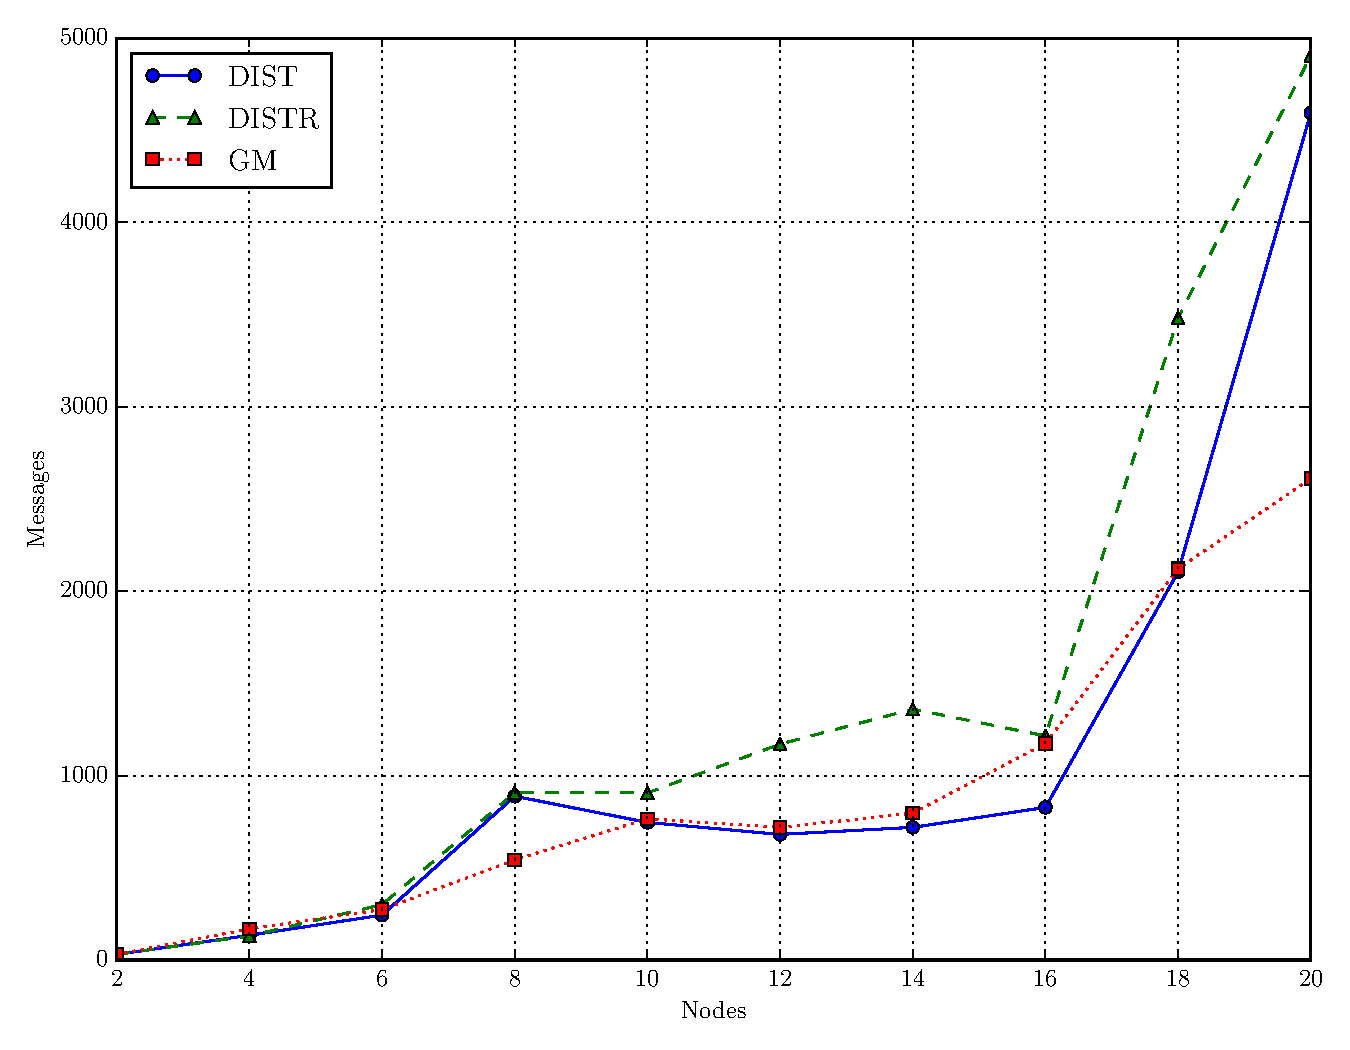
\includegraphics[width=\linewidth]{img/matching_msg_linear.pdf}
  \caption{Communication costs of methods RAND,DISTR and DIST for the \emph{LIN} dataset.}
\end{subfigure}\hfill
\begin{subfigure}{0.32\textwidth}
  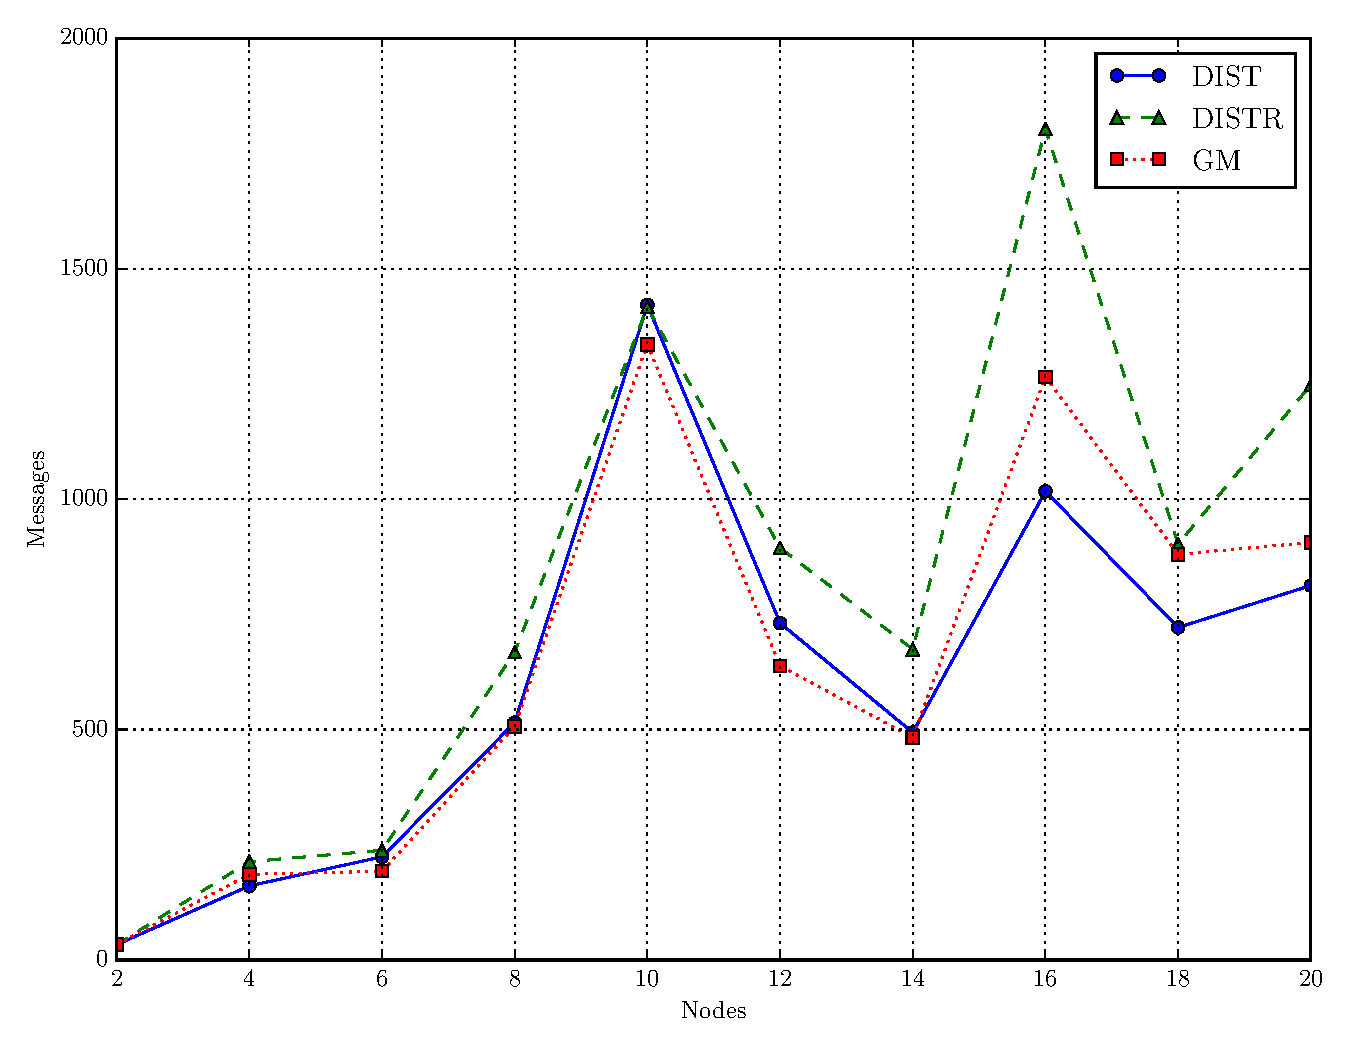
\includegraphics[width=\linewidth]{img/matching_msg_interweaving.pdf}
  \caption{Communication costs of methods RAND,DISTR and DIST for the \emph{INT} dataset.}
\end{subfigure}\hfill
\begin{subfigure}{0.32\textwidth}%
  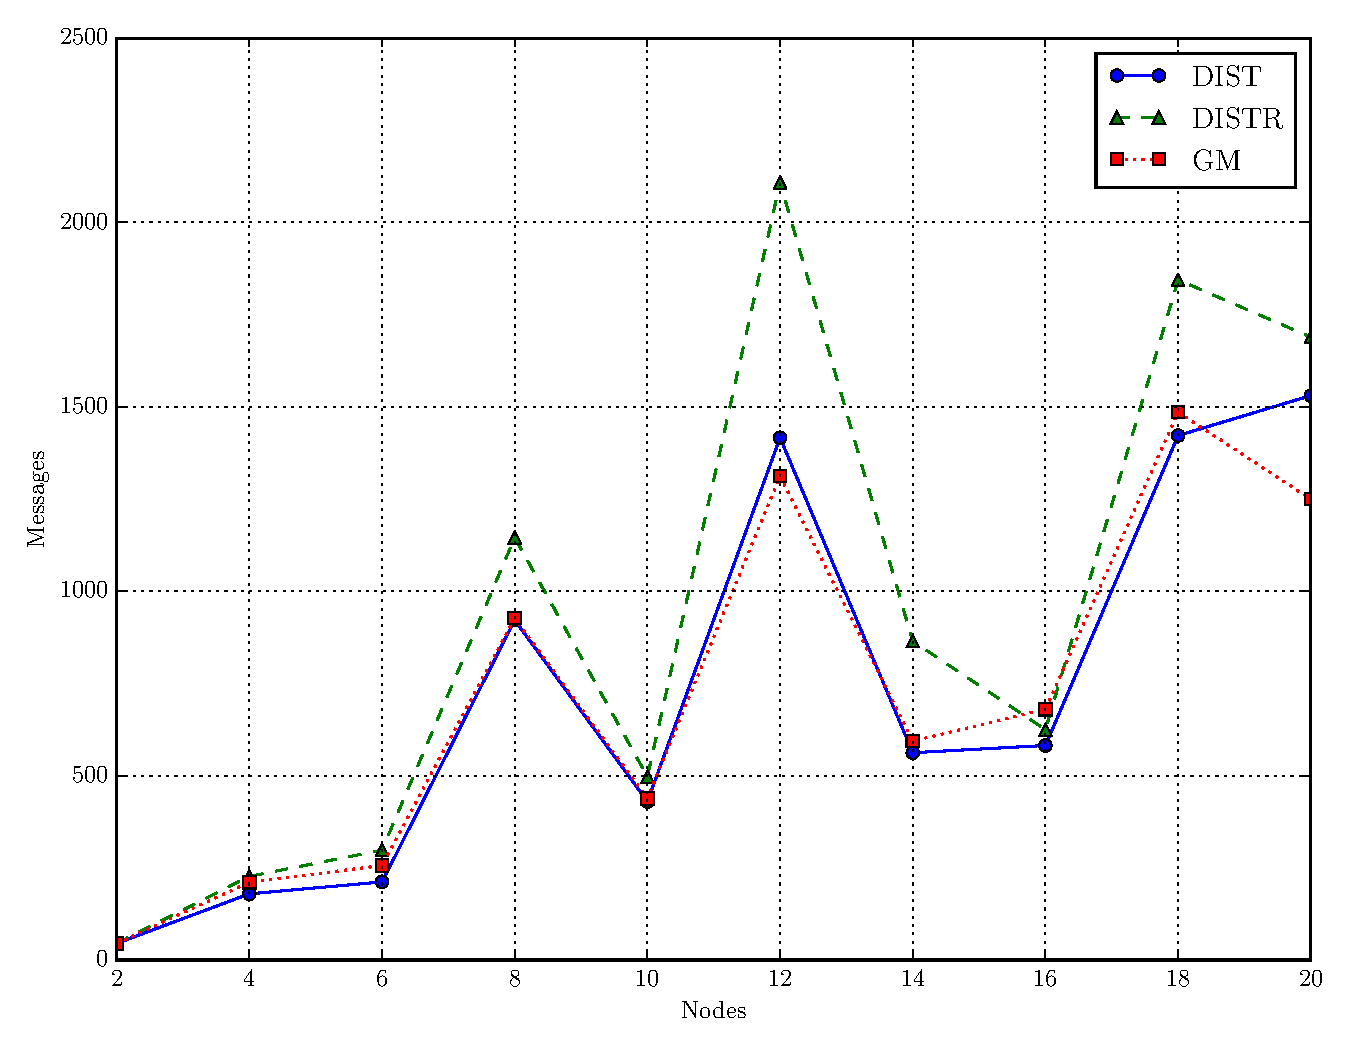
\includegraphics[width=\linewidth]{img/matching_msg_noisyinterweaving.pdf}
  \caption{Communication costs of methods RAND,DISTR and DIST for the \emph{NOISE} dataset.}
\end{subfigure}
\vspace{0.5cm}
\caption{Comparison of RAND, DISTR and DIST methods in terms of communication cost in messages over the range of 20 nodes.} \label{fig:matchingComp-msgs}
\end{figure}
%%%%%%%%%%%%%%%%%%%%%%%%%%%%%%%%%%%%%%%%%%%%%%%%%%%%%%%%%%%%%%%%%%%%%%%%%%%%%%%%%%%%%%%%%%%
%%%%%%%%%%%%%%%%%%%%%%%%%%%%%%%%drifts matching lin figure %%%%%%%%%%%%%%%%%%%%%%%%%%%%
\begin{figure}[!b]
\begin{subfigure}{0.32\textwidth}
  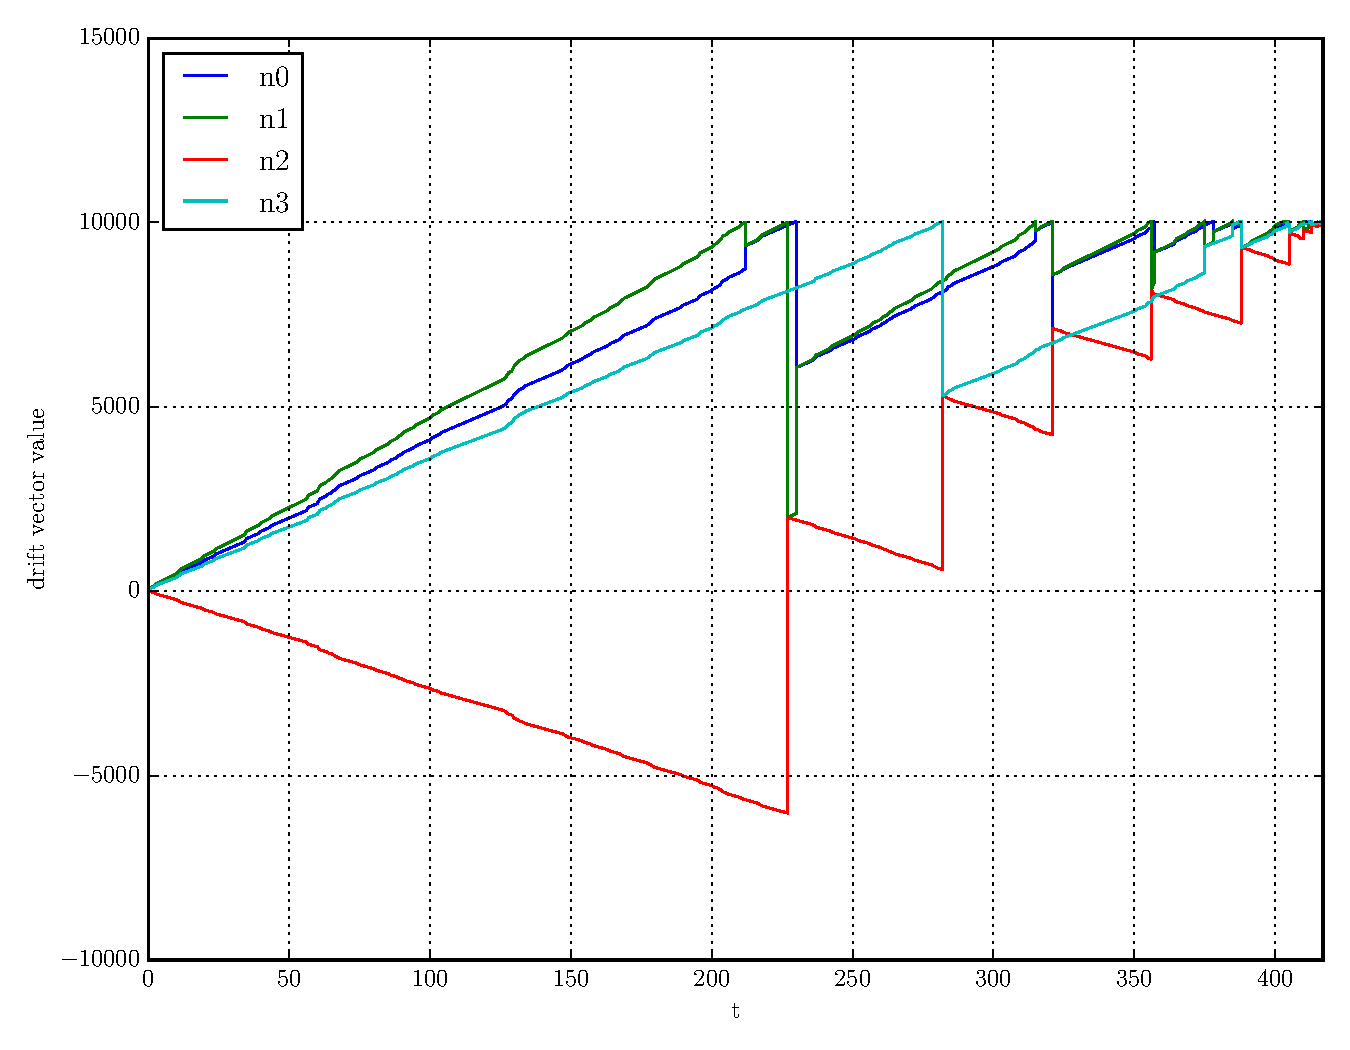
\includegraphics[width=\linewidth]{img/matchings_classic_random_drifts.pdf}
  \caption{Drift vectors of 4 nodes as a result of the RAND method.}
\end{subfigure}\hfill
\begin{subfigure}{0.32\textwidth}
  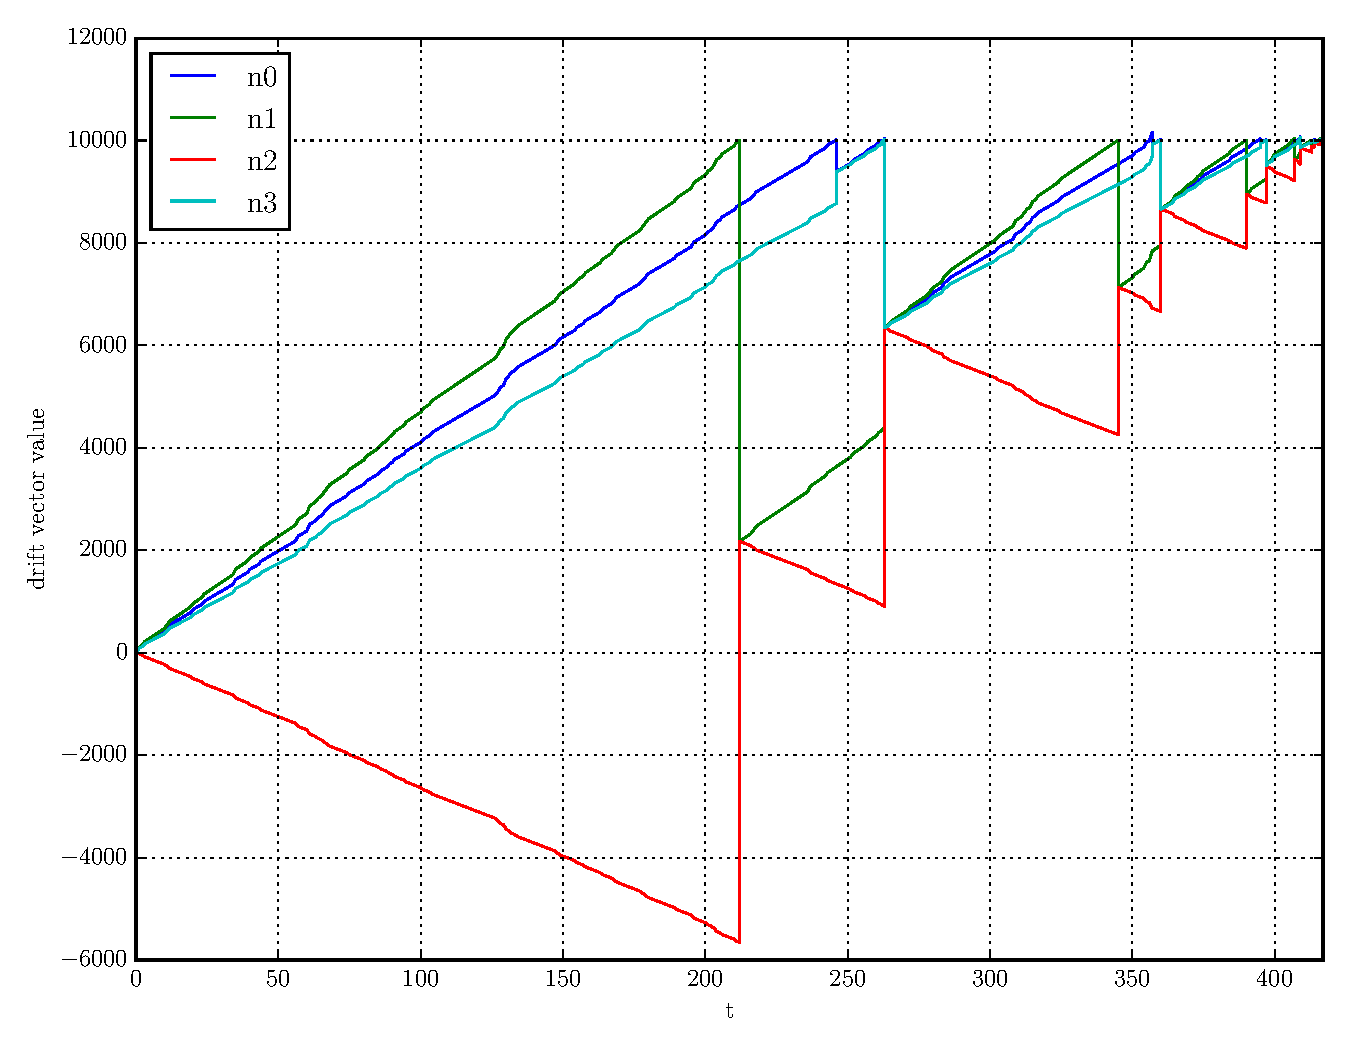
\includegraphics[width=\linewidth]{img/matchings_classic_distoptpair_drifts.pdf}
  \caption{Drift vectors of 4 nodes as a result of the DIST method.}
\end{subfigure}\hfill
\begin{subfigure}{0.32\textwidth}%
  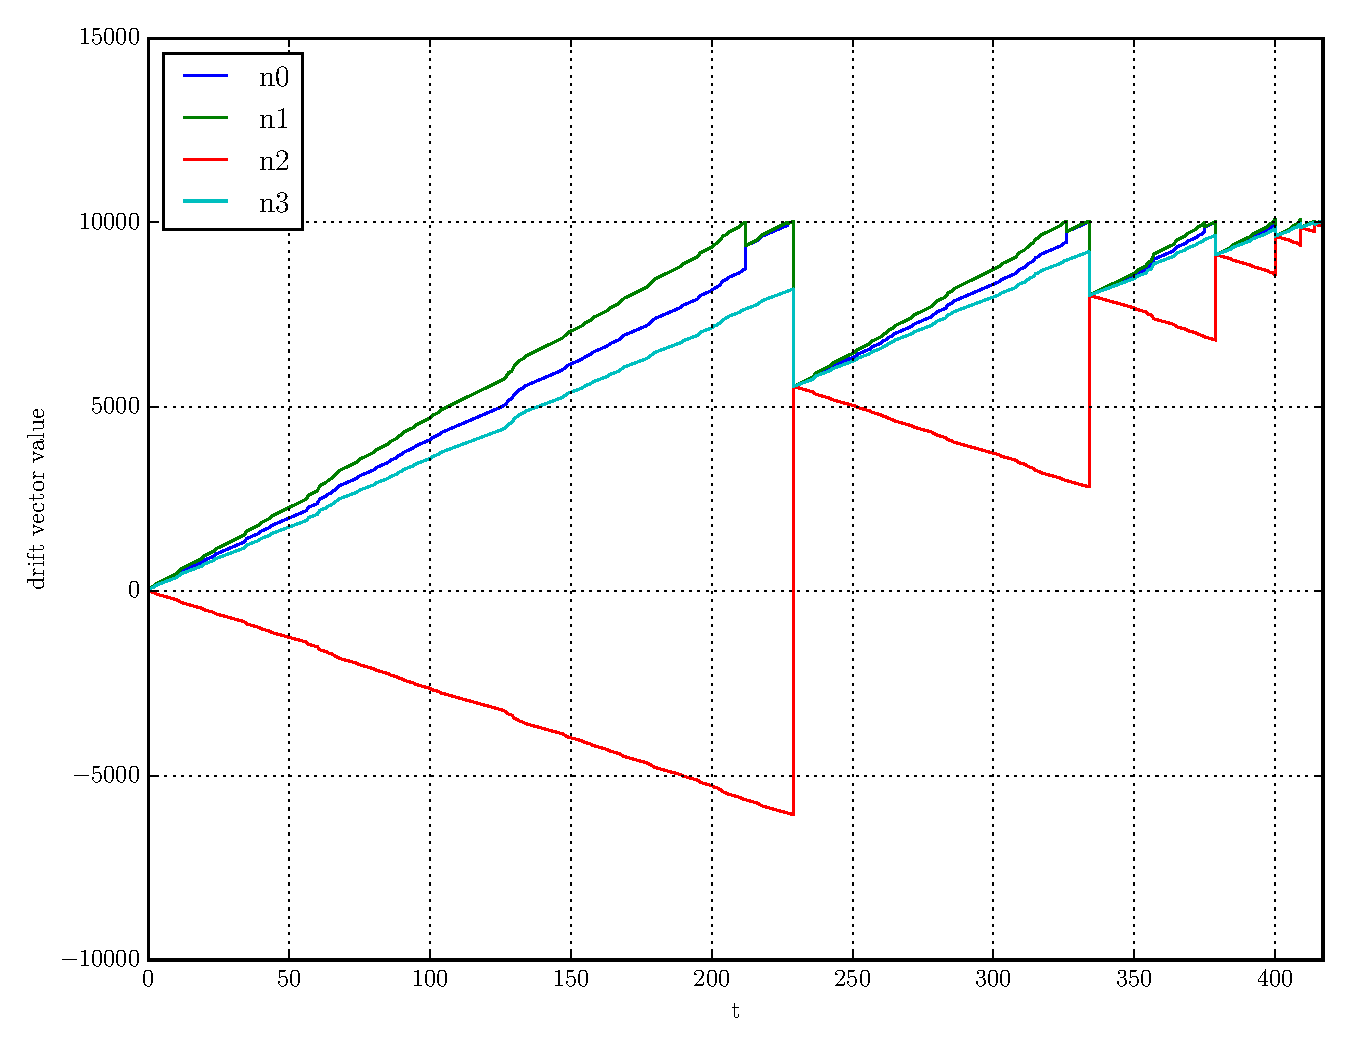
\includegraphics[width=\linewidth]{img/matchings_classic_distroptpair_drifts.pdf}
  \caption{Drift vectors of 4 nodes as a result of the DISTR method.}
\end{subfigure}
\vspace{0.5cm}
\caption{Drift vectors of 4 nodes as a result of application of RAND, DIST and DISTR methods over the \emph{LIN} dataset.} \label{fig:matchingComp-drifts}
\end{figure}
%%%%%%%%%%%%%%%%%%%%%%%%%%%%%%%%%%%%%%%%%%%%%%%%%%%%%%%%%%%%%%%%%%%%%%%%%%%%%%%%%%%%%%%%%%%
%%%%%%%%%%%%%%%%%%%%%%%%%%%%%%%%matchings matching lin figure %%%%%%%%%%%%%%%%%%%%%%%%%%%%
\begin{figure}[!ht]\centering
\vspace{-0.5cm}
\begin{subfigure}{\textwidth}
	\centering
  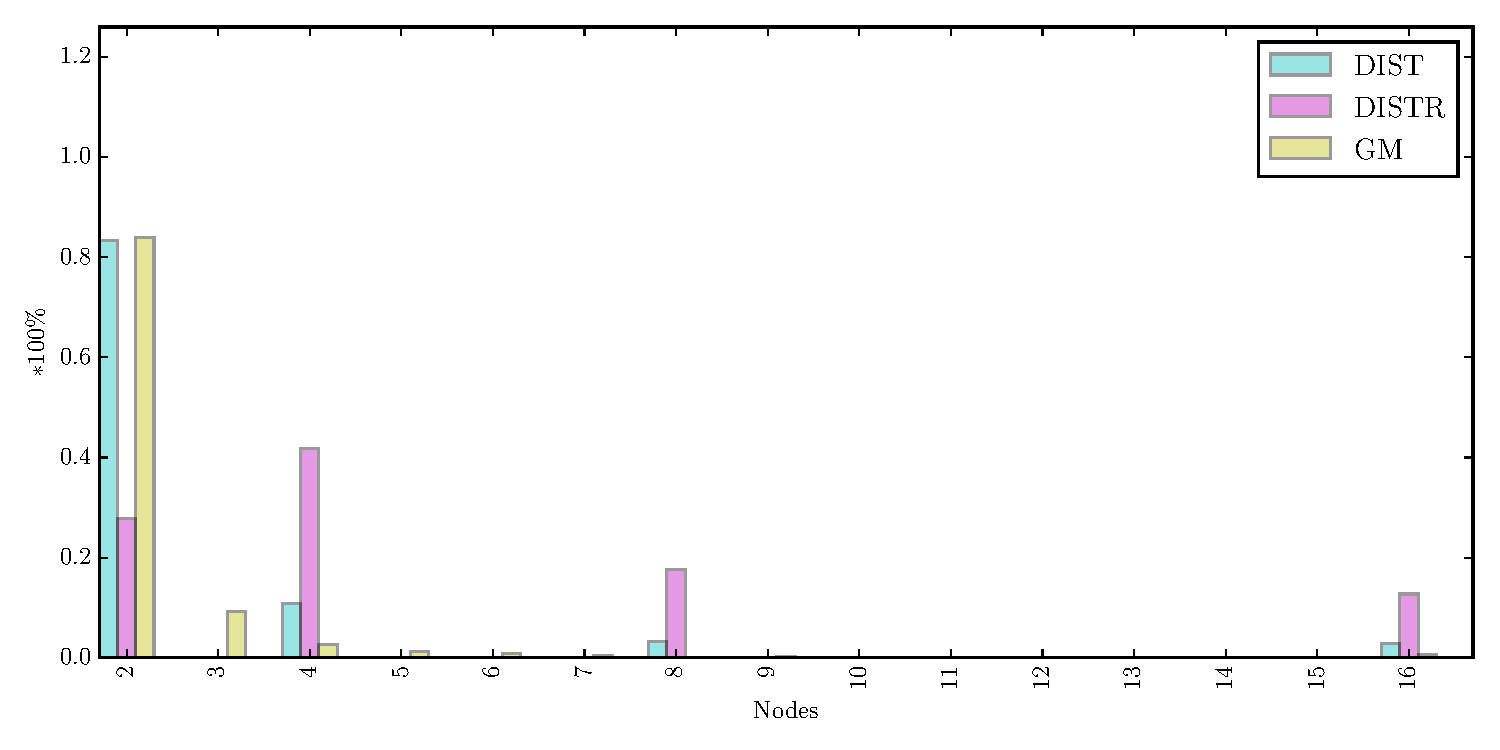
\includegraphics[width=0.72\linewidth]{img/matchings_matchings_linear.pdf}
  \caption{Number of nodes participating in violation resolutions as a fraction of total Local Violations, for the \emph{LIN} dataset.}
\end{subfigure}\hfill\\[1.5em]
\begin{subfigure}{\textwidth}
\centering
  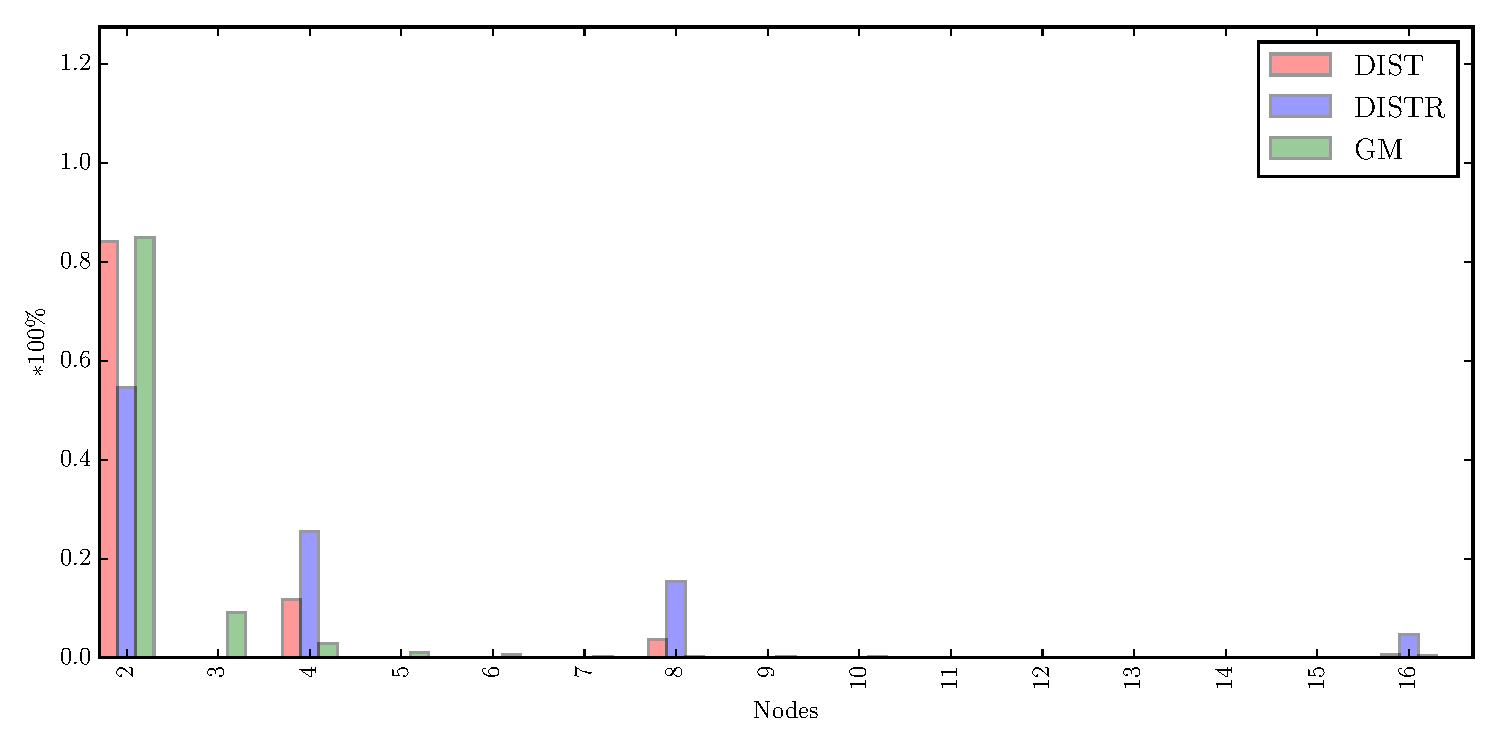
\includegraphics[width=0.72\linewidth]{img/matchings_matchings_interweaving.pdf}
  \caption{Number of nodes participating in violation resolutions as a fraction of total Local Violations, for the \emph{INT} dataset.}
\end{subfigure}\hfill\\[1.5em]
\begin{subfigure}{\textwidth}%
\centering
  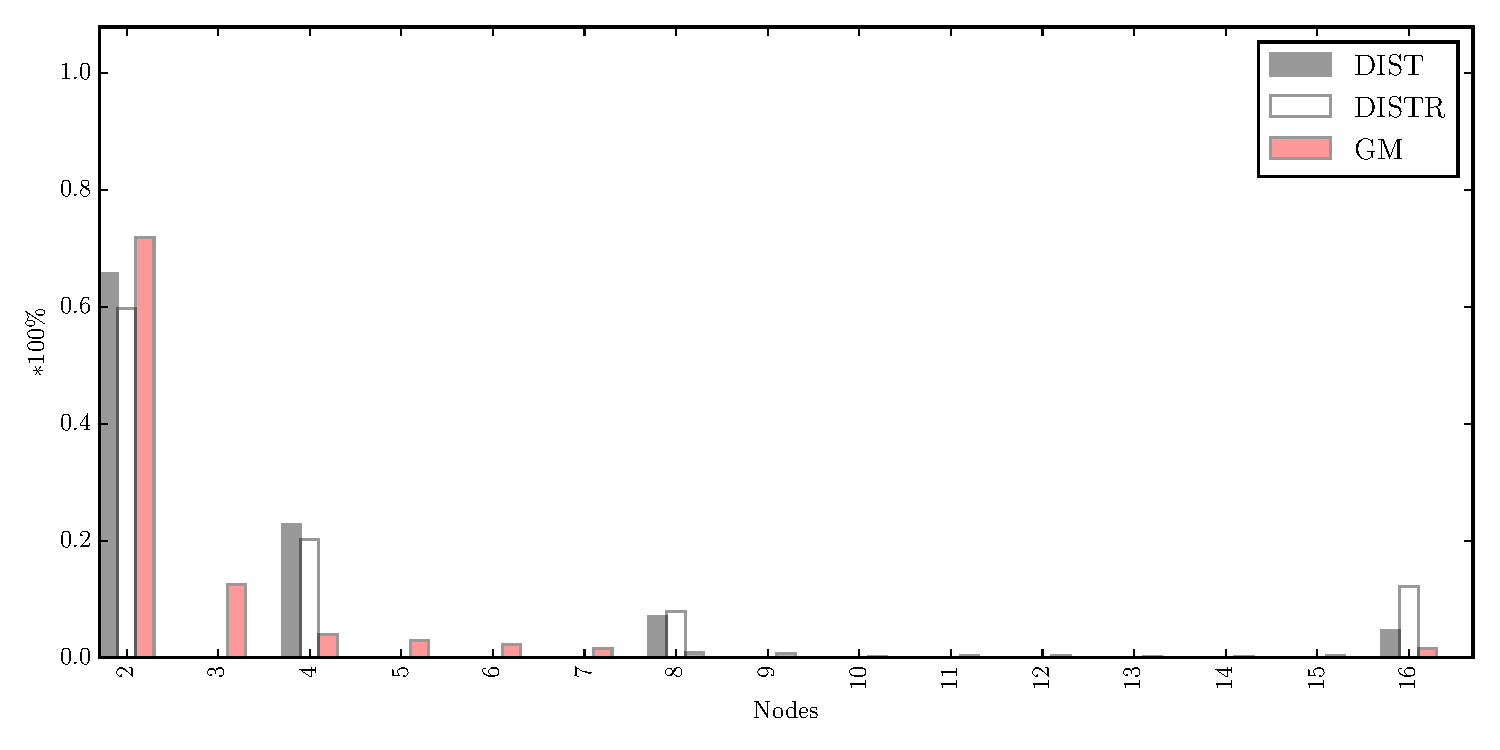
\includegraphics[width=0.72\linewidth]{img/matchings_matchings_noisyinterweaving.pdf}
  \caption{Number of nodes participating in violation resolutions as a fraction of total Local Violations, for the \emph{NOISE} dataset.}
\end{subfigure}
\vspace{0.5cm}
\caption{Number of nodes required to successfully resolve a violation, as a fraction of total Local Violations, for methods RAND, DISTR and DIST.} \label{fig:matchingComp-matchings}
\end{figure}
%%%%%%%%%%%%%%%%%%%%%%%%%%%%%%%%%%%%%%%%%%%%%%%%%%%%%%%%%%%%%%%%%%%%%%%%%%%%%%%%%%%%%

\subsection{Balancing methods} \label{subsec:balComp}

During the balancing process of the original geometric monitoring method~\cite{Sharfman2006GM} (GM) the computed drift vectors of the nodes are set to the value of the balancing vector that successfully resolves the reported Local Violation. In contrast, the heuristic balancing method proposed in this thesis (HM) attempts to optimize the positioning of the new drift vectors by taking into account the properties of each stream. Figure~\ref{fig:balComp-msgs} illustrates the communication cost induced by the balancing methods over a range of 2 to 20 nodes for the datasets \emph{LIN, INT} and \emph{NOISE}, when applied alongside the random node selection method (RAND) for violation resolution. For the HM method a window size of 10 and an approximation order of 1 are employed for the Savitzky-Golay filter.

%%%%%%%%%%%%%%%%%%%%%%%%%%%%%%%%msgs bal  figure %%%%%%%%%%%%%%%%%%%%%%%%%%%%
\begin{figure}[!h]
\begin{subfigure}{0.32\textwidth}
  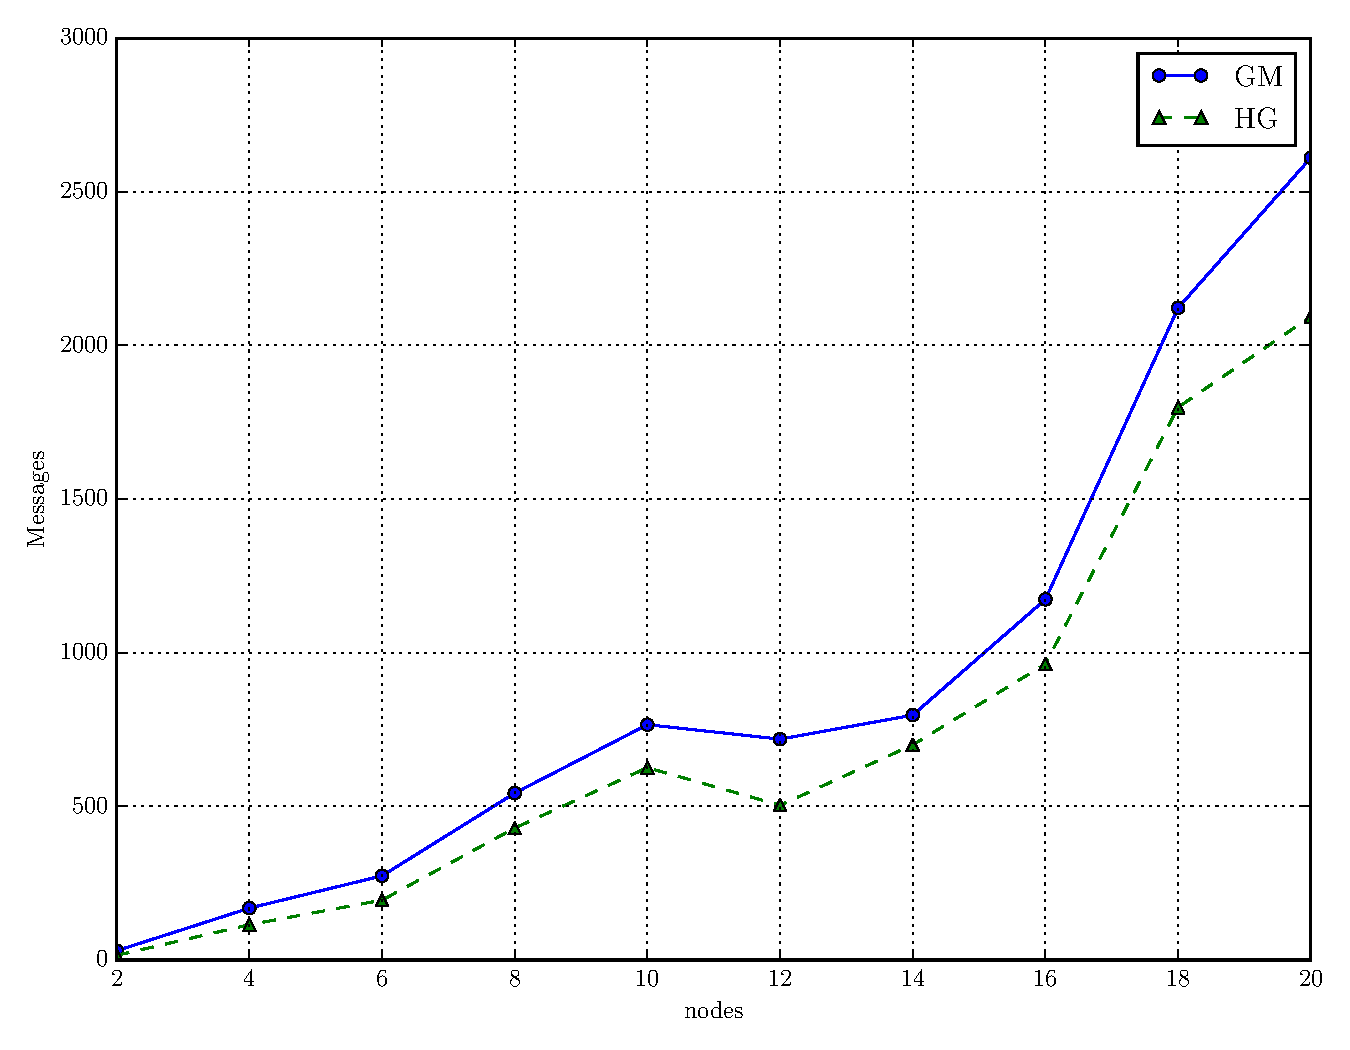
\includegraphics[width=\linewidth]{img/bal_msg_linear_nodes.pdf}
  \caption{Communication cost of methods GM and HM for the \emph{LIN} dataset.}
\end{subfigure}\hfill
\begin{subfigure}{0.32\textwidth}
  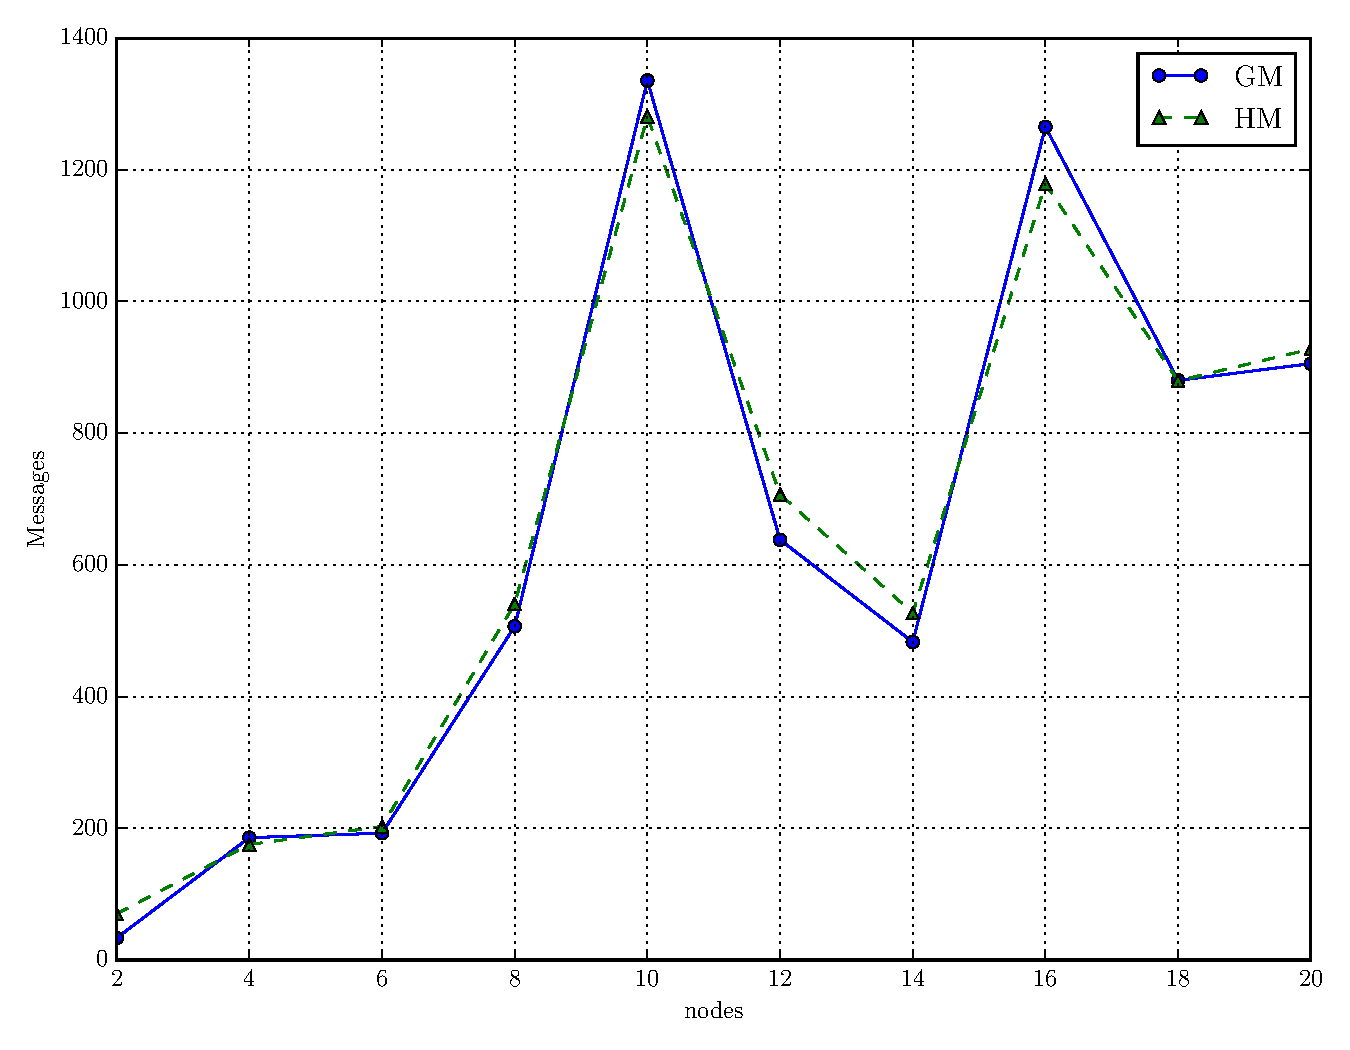
\includegraphics[width=\linewidth]{img/bal_msg_interweaving_nodes.pdf}
  \caption{Communication cost of methods GM and HM for the \emph{INT} dataset.}
\end{subfigure}\hfill
\begin{subfigure}{0.32\textwidth}%
  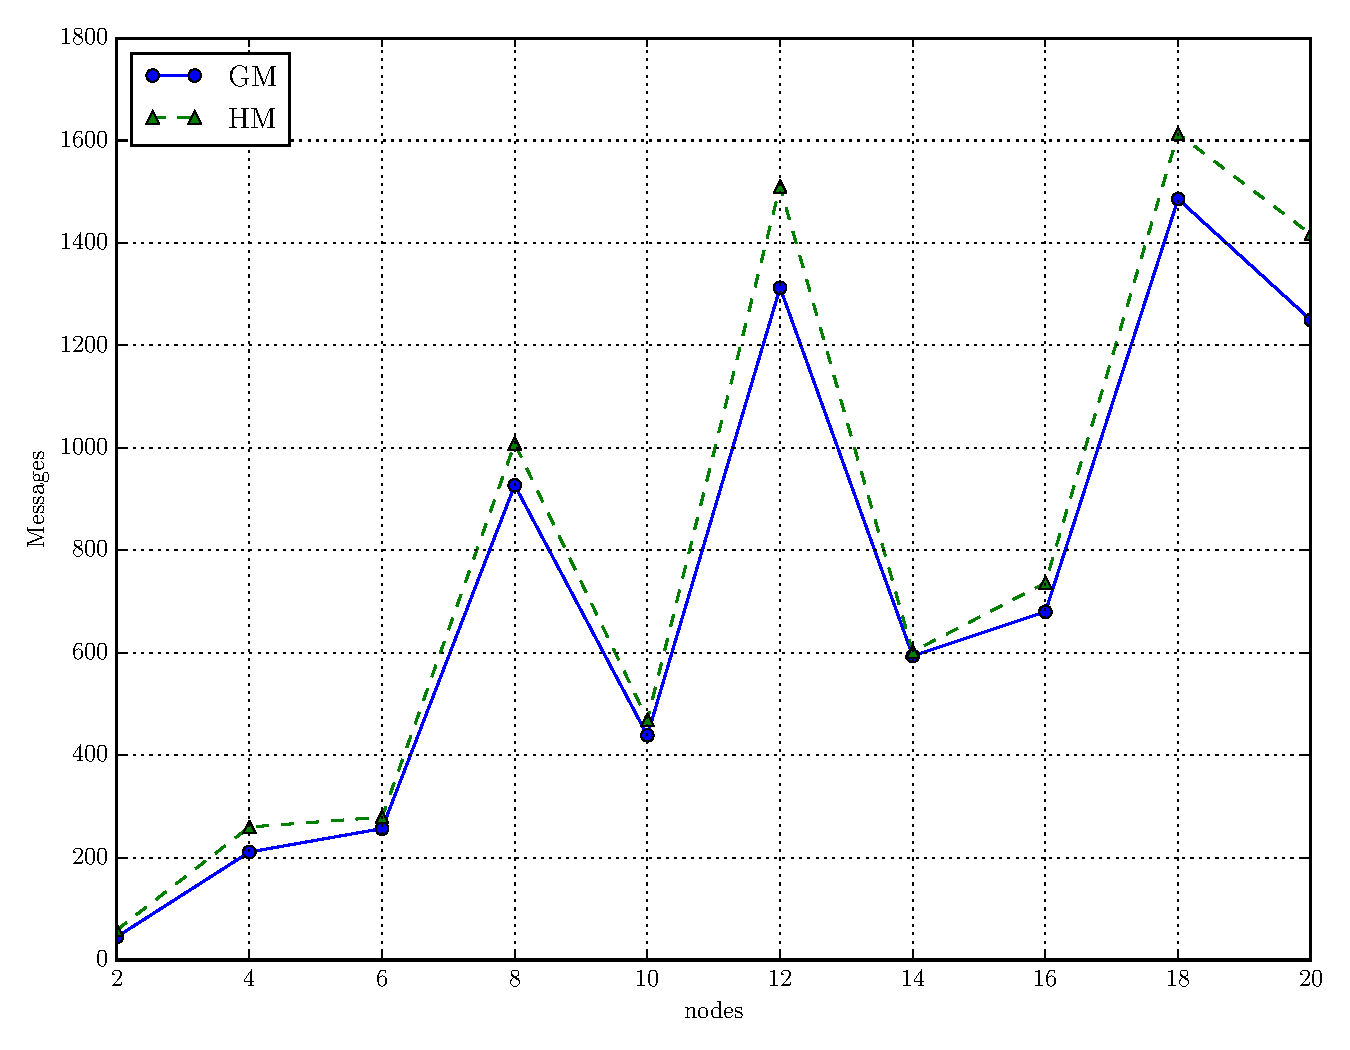
\includegraphics[width=\linewidth]{img/bal_msg_noisyinterweaving_nodes.pdf}
  \caption{Communication cost of methods GM and HM for the \emph{NOISE} dataset.}
\end{subfigure}
\vspace{0.5cm}
\caption{Comparison of the GM and HM methods in terms of communication cost over a range of 20 nodes. For the Savitzky-Golay filter of HM method a window size of 10 and an order of 1 are employed.} \label{fig:balComp-msgs}
\end{figure}
%%%%%%%%%%%%%%%%%%%%%%%%%%%%%%%%%%%%%%%%%%%%%%%%%%%%%%%%%%%%%%%%%%%%%%%%%%%%%%%%%%%%%%%%%%%

When applied to the \emph{LIN} dataset the HM method consistently surpasses the original GM balancing method in terms of communication reduction by optimally positioning the drift vectors following a Local Violation resolution, a property illustrated in Figure~\ref{fig:balComp-drifts} for 2 monitoring nodes. When data streams become more complex and unpredictable, i.e., the \emph{INT} and \emph{NOISE} datasets, the HM method provides a similar to slightly worse performance than that of GM, due to variable velocities and accelerations affecting the performance of the optimization function. Additionally, the selection of random nodes at each resolution attempt hampers the performance of HM due to the fact that optimal positioning computation is relative to the nodes taking part in a specific balancing process. Thus, when an optimized drift vector participates in a subsequent balancing process with a different node set the existing optimization and the ``correlation'' between optimized sets is discarded.

%%%%%%%%%%%%%%%%%%%%%%%%%%%%%%%%drifts bal lin figure %%%%%%%%%%%%%%%%%%%%%%%%%%%%
\begin{figure}[!h]
\begin{subfigure}{0.49\textwidth}
  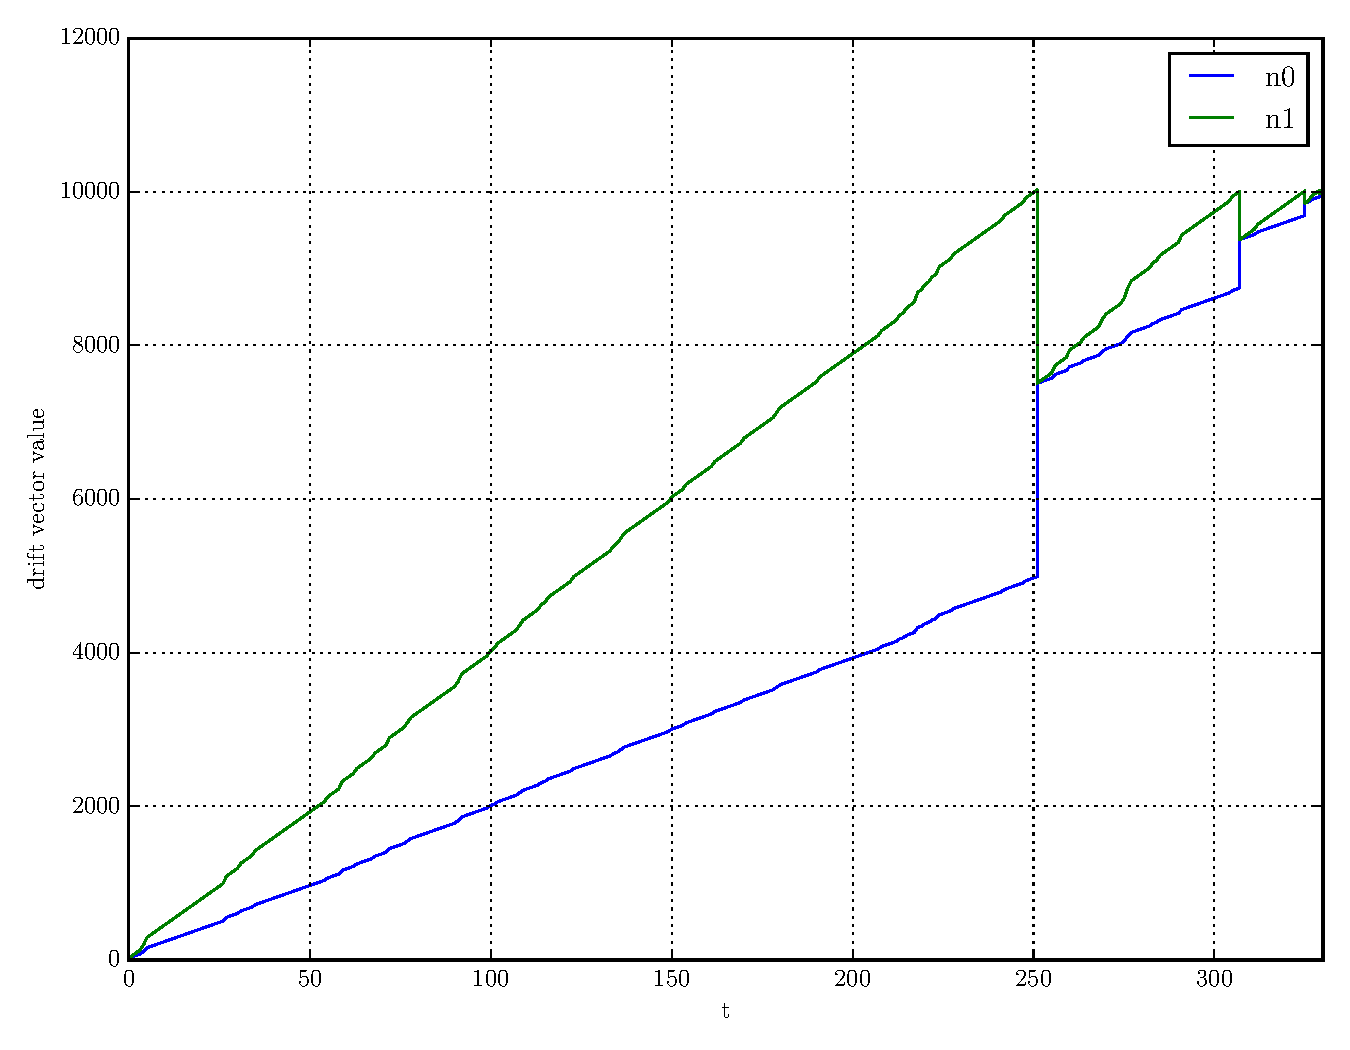
\includegraphics[width=\linewidth]{img/bal_classic_drifts_linear2N.pdf}
  \caption{Drift vectors of 2 nodes, as formulated by the GM algorithm.}
\end{subfigure}\hfill
\begin{subfigure}{0.49\textwidth}
  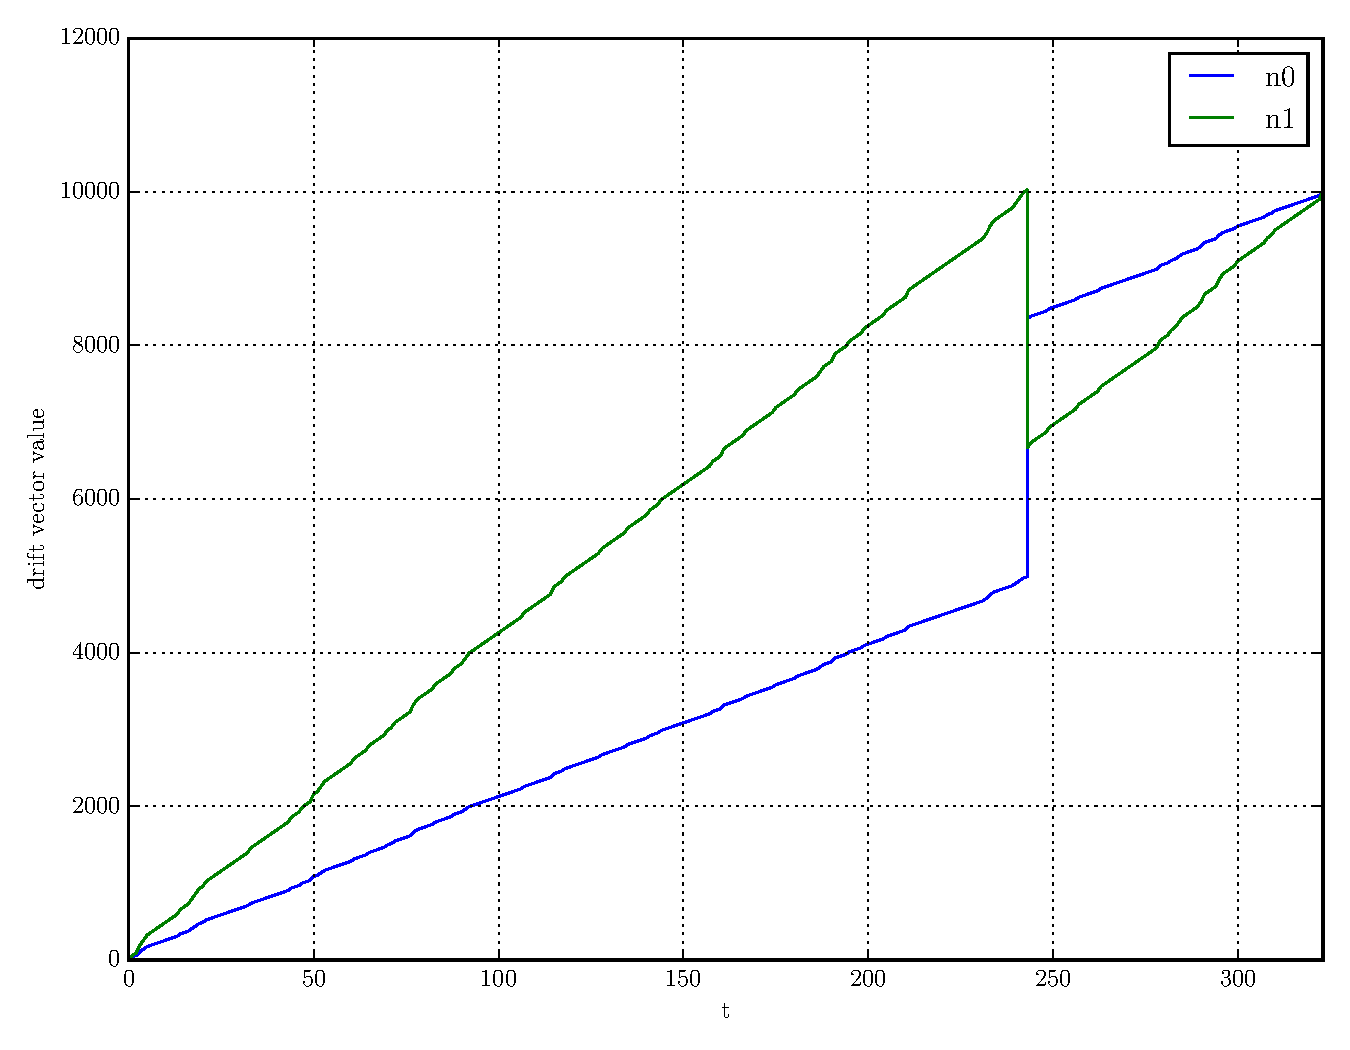
\includegraphics[width=\linewidth]{img/bal_heuristic_drifts_linear2N.pdf}
  \caption{Drift vectors of 2 nodes, as formulated by the HM algorithm.}
\end{subfigure}\hfill
\vspace{0.5cm}
\caption{The drift vectors of 2 nodes with streams originating from the \emph{LIN} dataset, when the GM and HM balancing methods are applied.} \label{fig:balComp-drifts}
\end{figure}
%%%%%%%%%%%%%%%%%%%%%%%%%%%%%%%%%%%%%%%%%%%%%%%%%%%%%%%%%%%%%%%%%%%%%%%%%%%%%%%%%%%%%%%%%%%

\subsection{Monitoring Synthetic Data} \label{subsec:mainComp}

In order to eliminate the unpredictability the RAND method incurs to HM, we compare the GM method with a combination of our proposed methods (DIST, HM), resulting to the HDM method. Figure~\ref{fig:mainComp-msgs} depicts the performance of the two methods over a range of 2 to 20 nodes, in terms of communication cost. Following that, Figures~\ref{fig:mainComp-order} and~\ref{fig:mainComp-wl} examine the way the Savitzky-Golay filter parameters affect the performance of HDM. Finally, Figure~\ref{fig:mainComp-dims} illustrates the scalability of the HDM method compared to the GM method, in terms of communication cost and stream dimensionality.

Once again, the HDM method outperforms the original GM method when applied onto the \emph{LIN} dataset for any parameter setting of the Savitzky-Golay filter by achieving a communication reduction of up to 60 percent. When datasets in the likes of \emph{INT} and \emph{NOISE} are employed, where smooth and drastic velocity changes can be observed, respectively, fine-tuning the filter's parameters can reduce the communication burden of HDM significantly, surpassing the GM algorithm in terms of communication reduction, as shown in Figures~\ref{fig:mainComp-order} and~\ref{fig:mainComp-wl}. Finally, when multiple stream dimensions are monitored the HDM method illustrates similar performance as with its one-dimensional stream counterparts.

%%%%%%%%%%%%%%%%%%%%%%%%%%%%%%%%msgs main  figure %%%%%%%%%%%%%%%%%%%%%%%%%%%%
\begin{figure}[!h]
\begin{subfigure}{0.32\textwidth}
  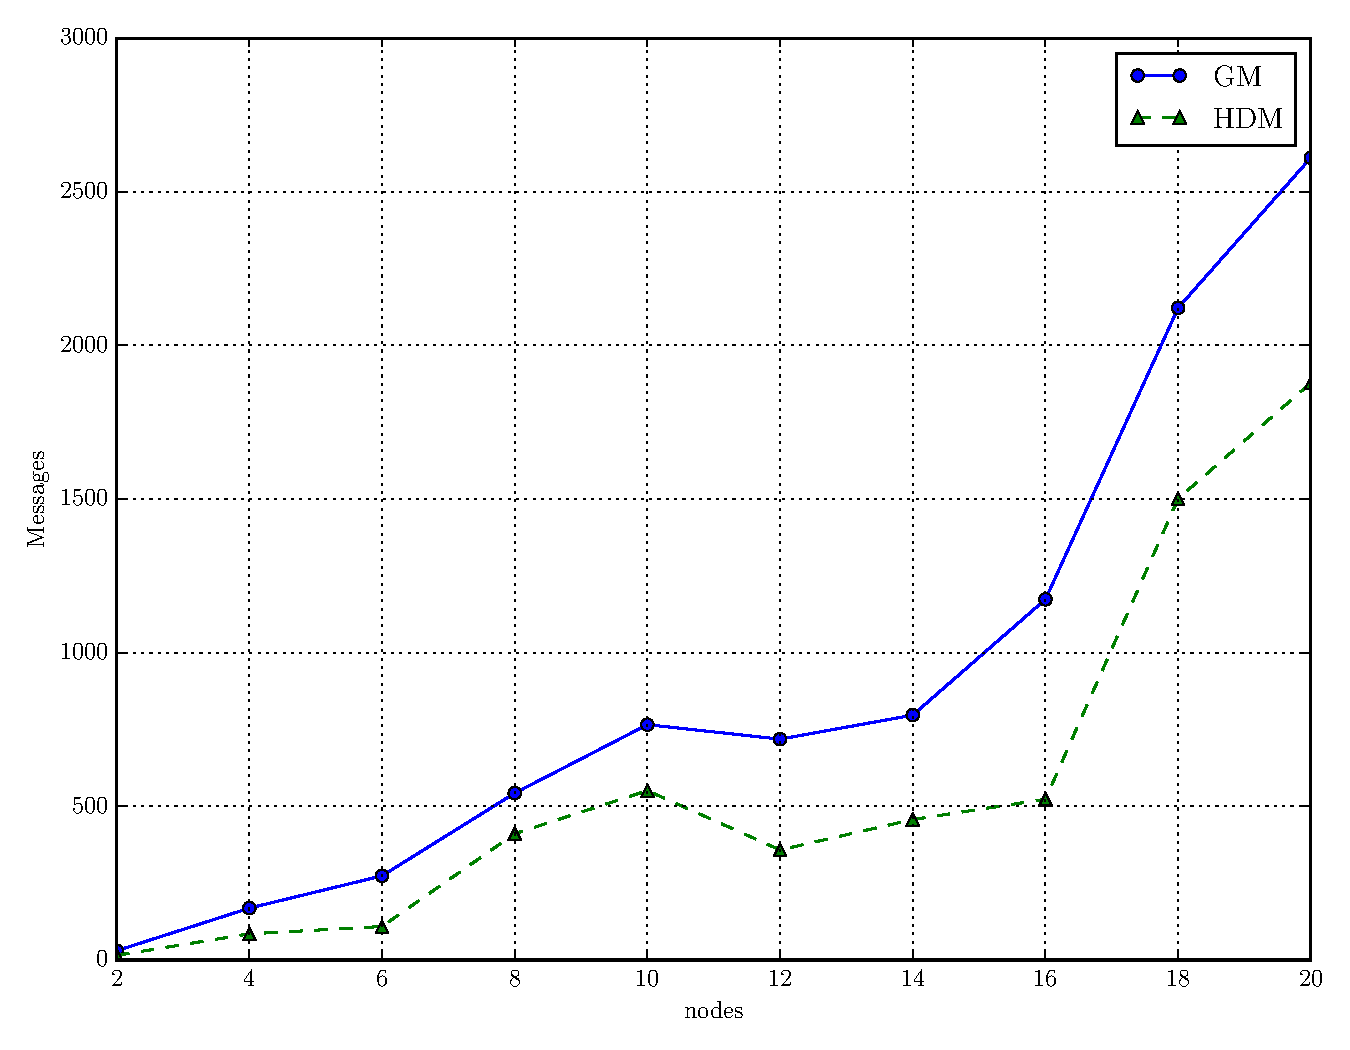
\includegraphics[width=\linewidth]{img/main_msg_linear_nodes.pdf}
  \caption{Communication cost of methods GM and HDM for the \emph{LIN} dataset. The Savitzky-Golay window size is set to 10 and the approximation order is set to 1.}
\end{subfigure}\hfill
\begin{subfigure}{0.32\textwidth}
  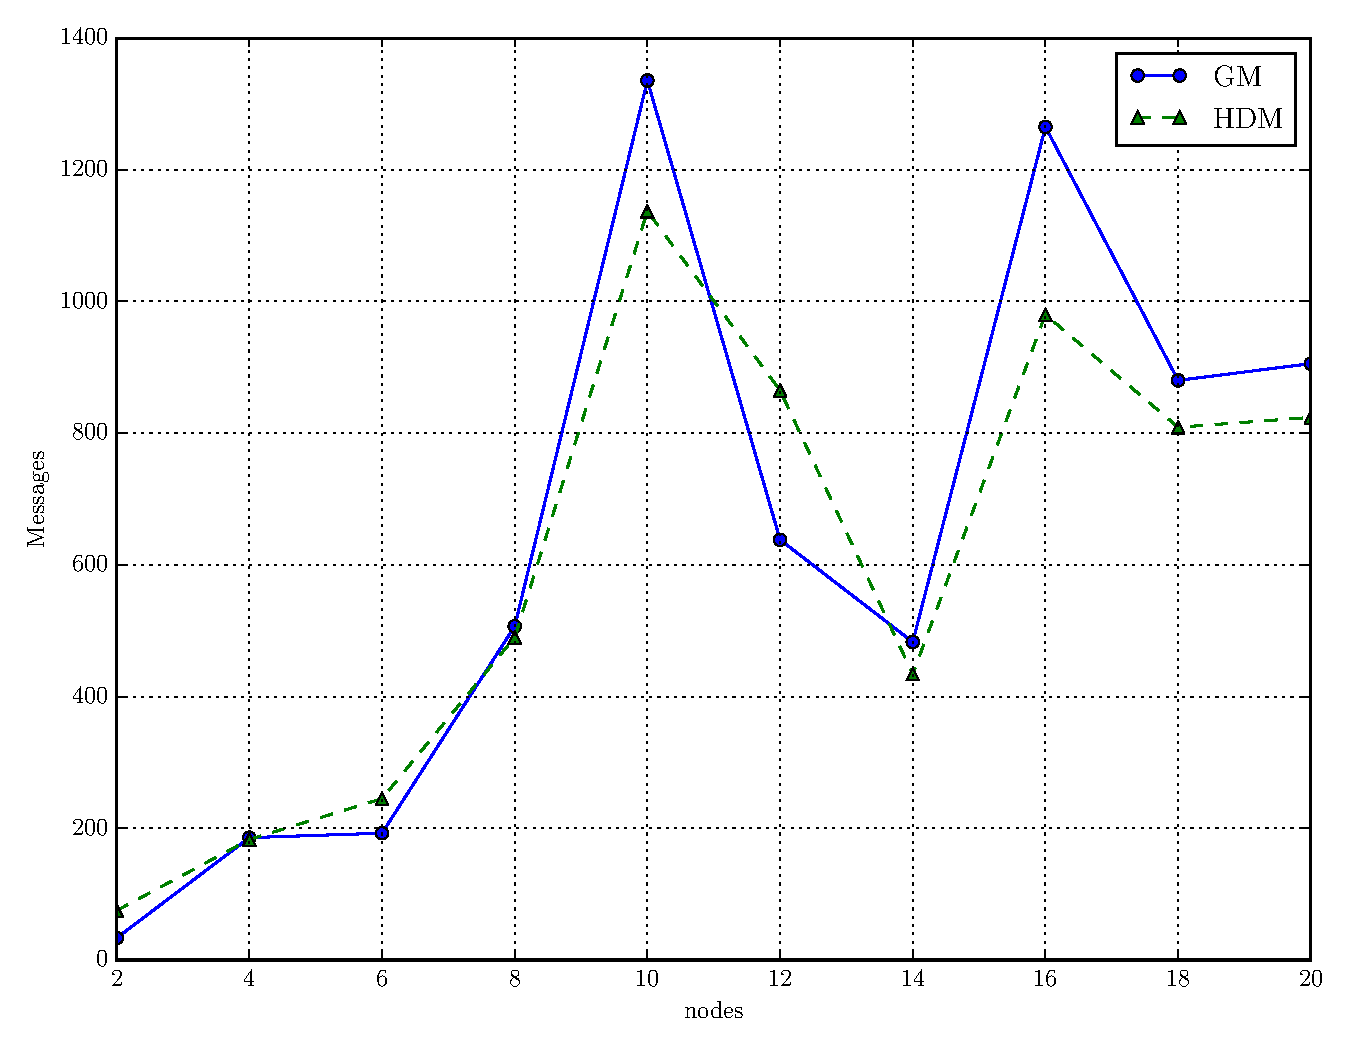
\includegraphics[width=\linewidth]{img/main_msg_interweaving_nodes.pdf}
  \caption{Communication cost of methods GM and HDM for the \emph{INT} dataset. The Savitzky-Golay window size is set to 10 and the approximation order is set to 1.}
\end{subfigure}\hfill
\begin{subfigure}{0.32\textwidth}%
  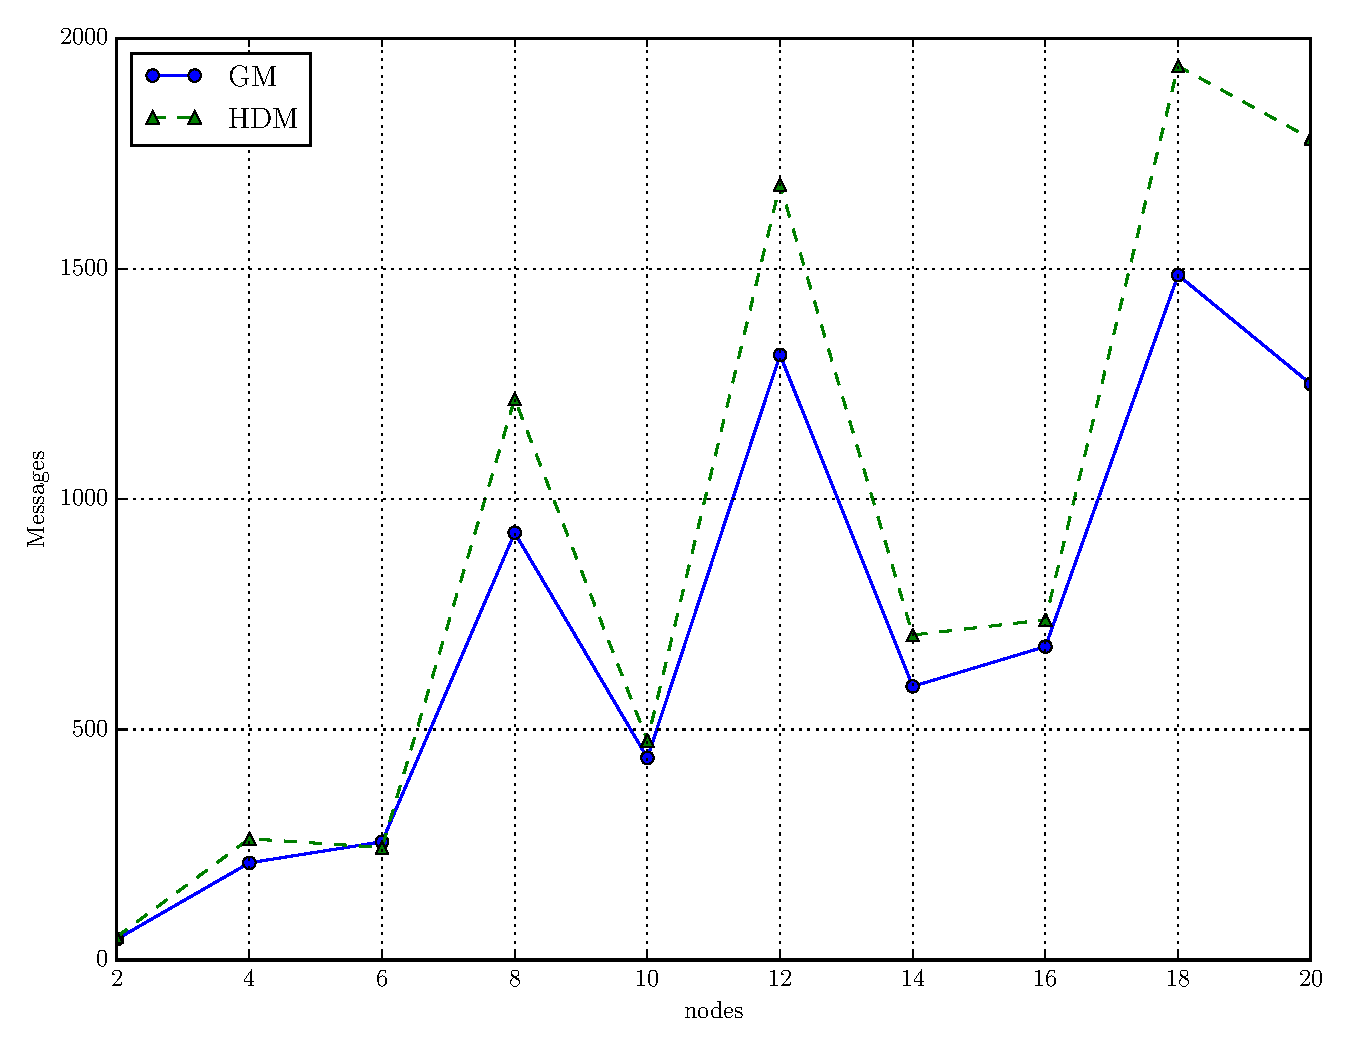
\includegraphics[width=\linewidth]{img/main_msg_noisyinterweaving_nodes.pdf}
  \caption{Communication cost of methods GM and HDM for the \emph{NOISE} dataset. The Savitzky-Golay window size is set to 24 and the approximation order is set to 1.}
\end{subfigure}
\vspace{0.5cm}
\caption{Comparison of the GM and HDM methods in terms of communication cost over a range of 20 nodes.} \label{fig:mainComp-msgs}
\end{figure}
%%%%%%%%%%%%%%%%%%%%%%%%%%%%%%%%%%%%%%%%%%%%%%%%%%%%%%%%%%%%%%%%%%%%%%%%%%%%%%%%%%%%%%%%%%%

%%%%%%%%%%%%%%%%%%%%%%%%%%%%%%%%wl main  figure %%%%%%%%%%%%%%%%%%%%%%%%%%%%
\begin{figure}[!h]
\begin{subfigure}{0.32\textwidth}
  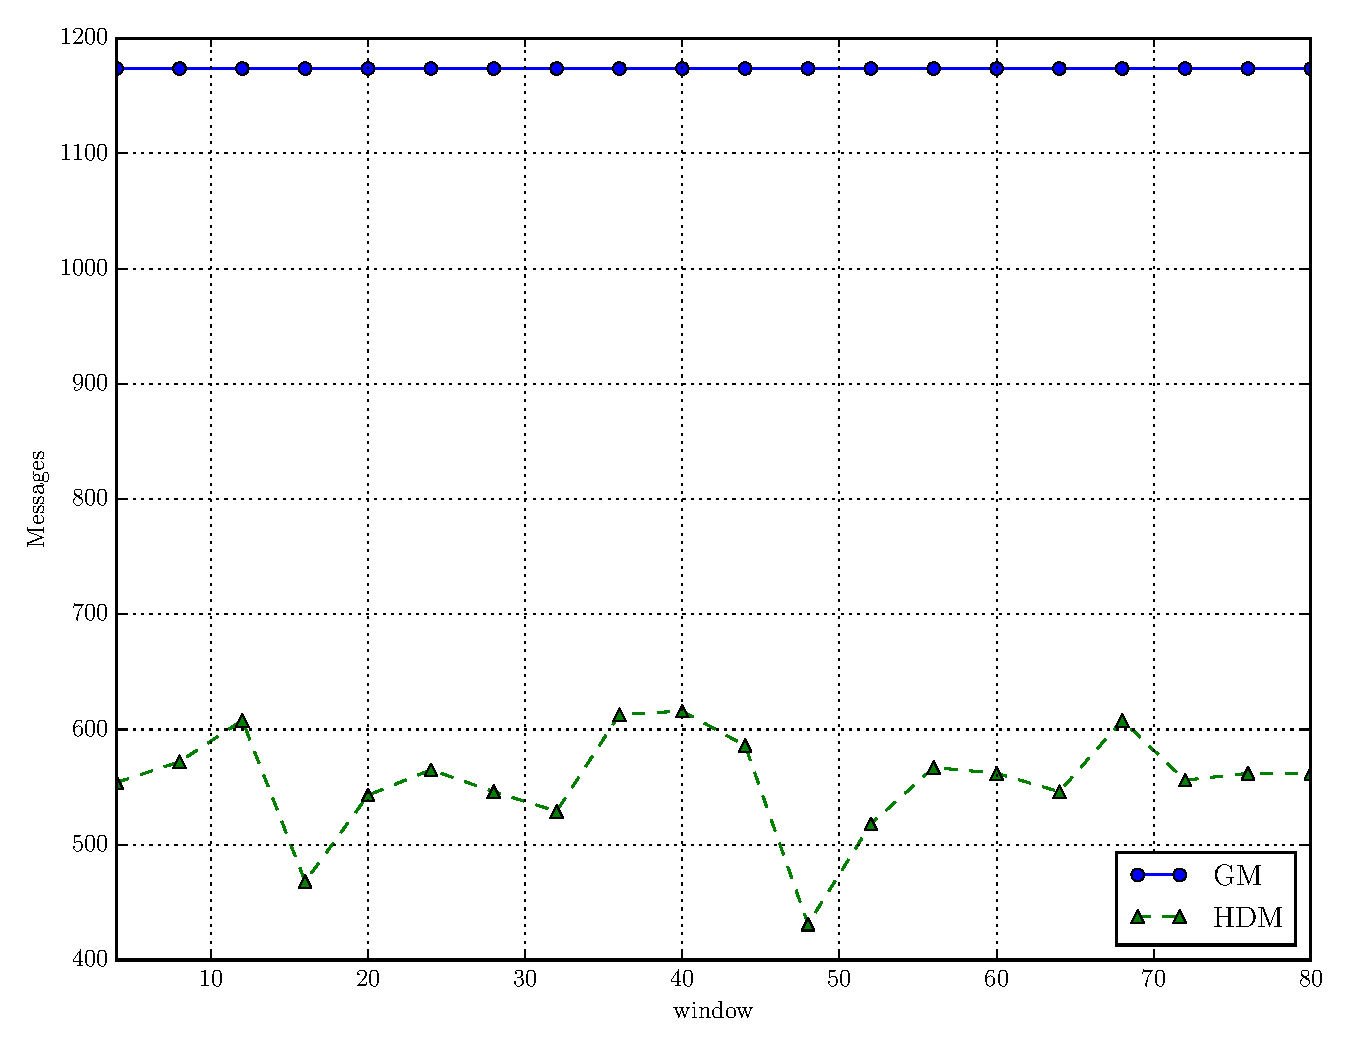
\includegraphics[width=\linewidth]{img/main_msg_linear_window.pdf}
  \caption{Communication cost of methods GM and HDM for the \emph{LIN} dataset.}
\end{subfigure}\hfill
\begin{subfigure}{0.32\textwidth}
  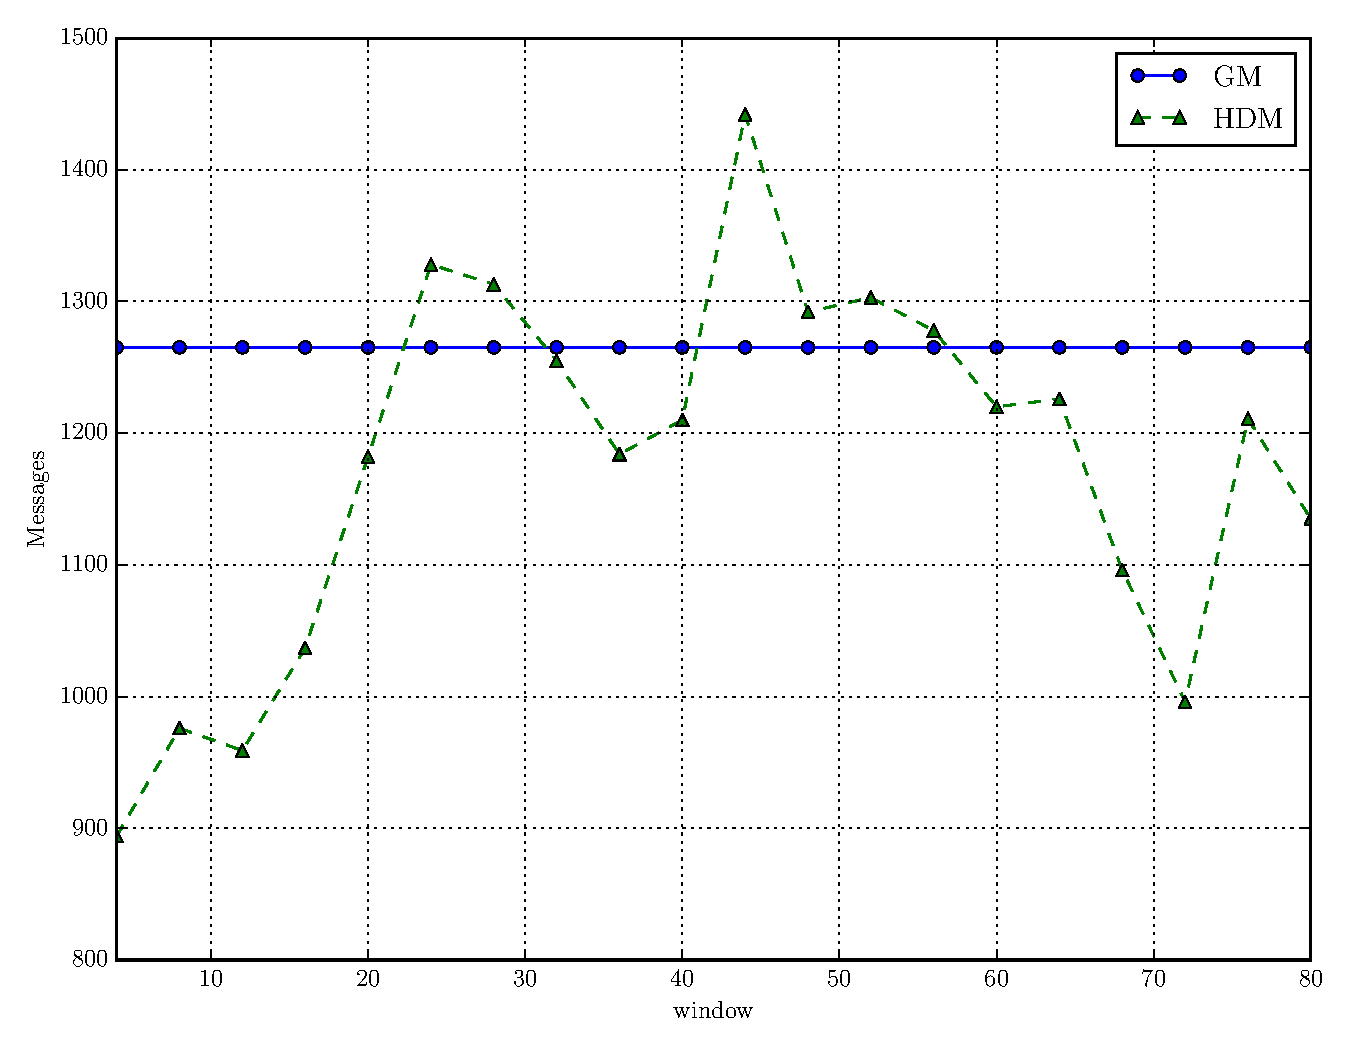
\includegraphics[width=\linewidth]{img/main_msg_interweaving_window.pdf}
  \caption{Communication cost of methods GM and HDM for the \emph{INT} dataset.}
\end{subfigure}\hfill
\begin{subfigure}{0.32\textwidth}%
  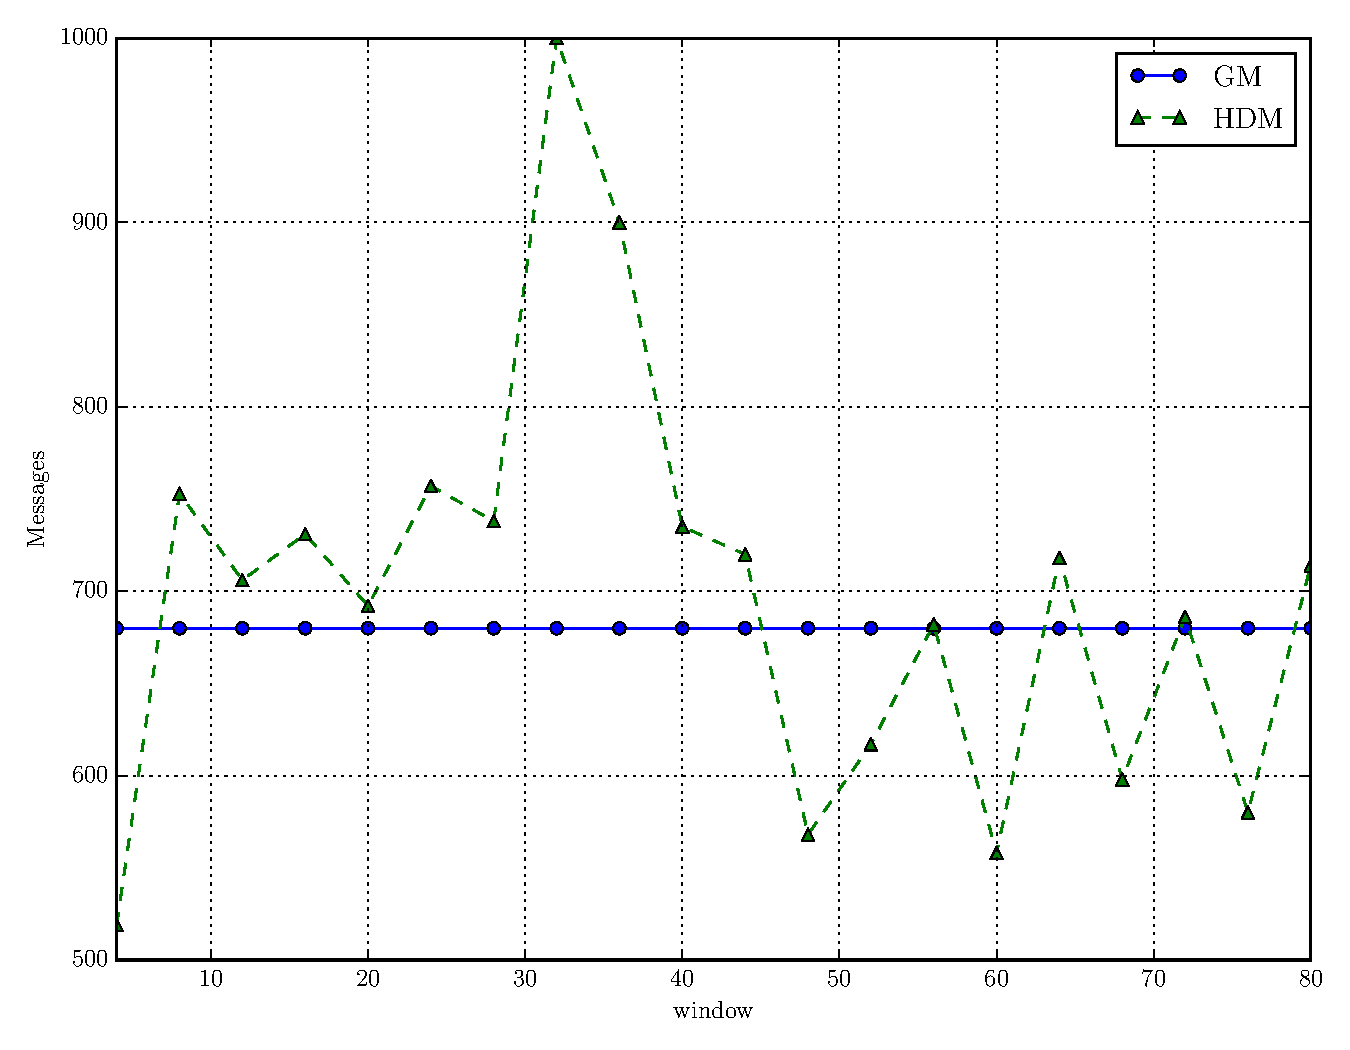
\includegraphics[width=\linewidth]{img/main_msg_noisyinterweaving_window.pdf}
  \caption{Communication cost of methods GM and HDM for the \emph{NOISE} dataset.}
\end{subfigure}
\vspace{0.5cm}
\caption{Comparison of the GM and HDM methods in terms of communication cost over a range of window sizes, for 16 nodes. The approximation order is set to 1 for all experiments.} \label{fig:mainComp-wl}
\end{figure}
%%%%%%%%%%%%%%%%%%%%%%%%%%%%%%%%%%%%%%%%%%%%%%%%%%%%%%%%%%%%%%%%%%%%%%%%%%%%%%%%%%%%%%%%%%%

%%%%%%%%%%%%%%%%%%%%%%%%%%%%%%%%order main  figure %%%%%%%%%%%%%%%%%%%%%%%%%%%%
\begin{figure}[!h]
\begin{subfigure}{0.32\textwidth}
  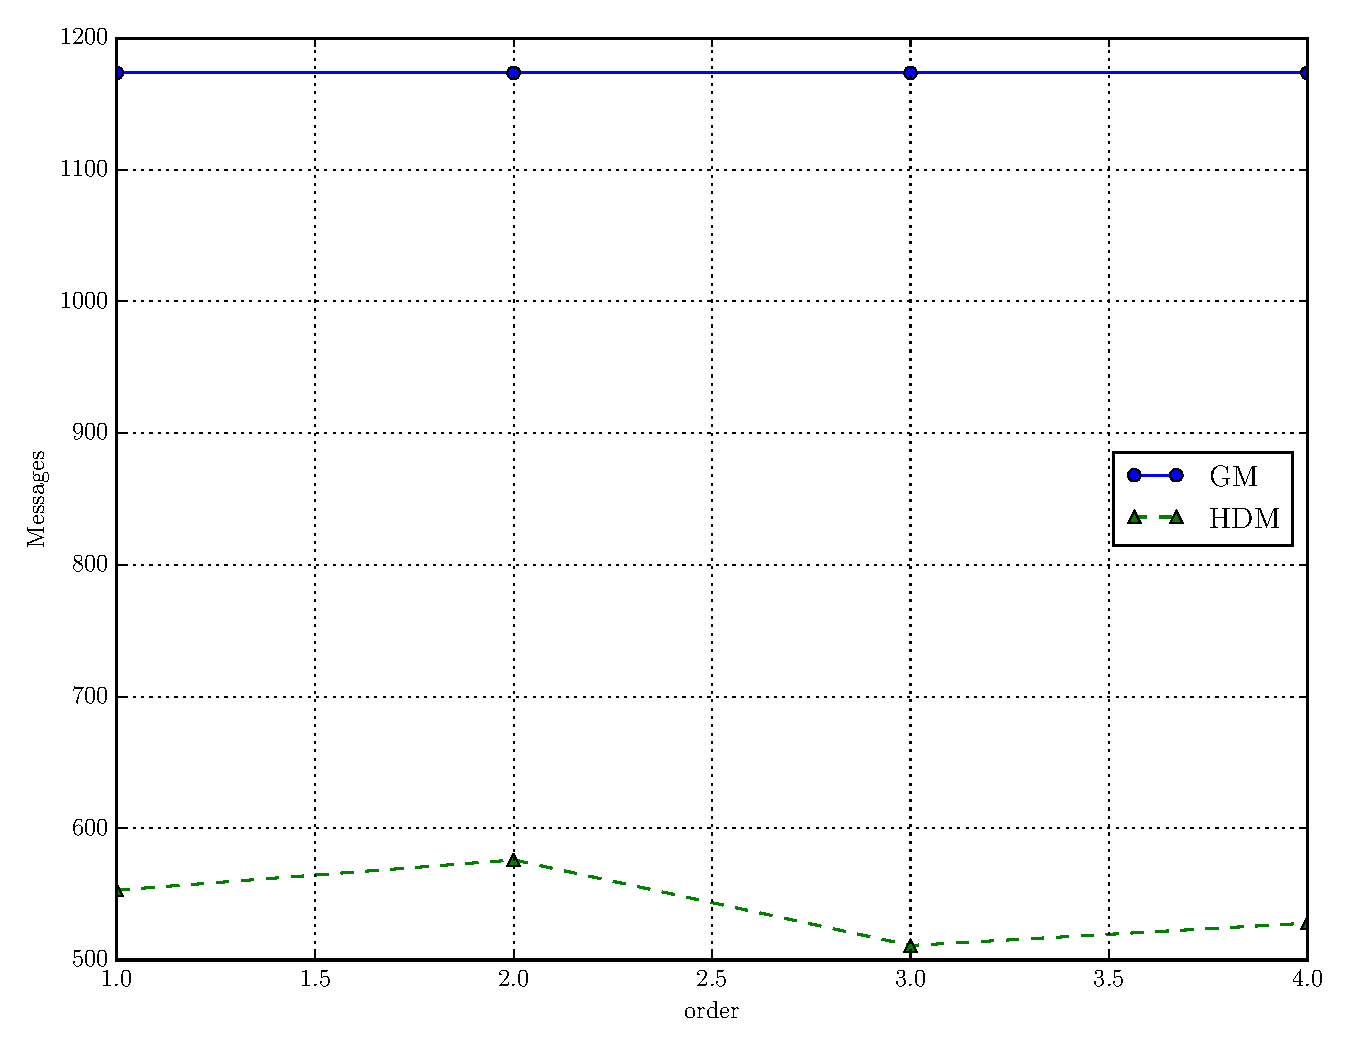
\includegraphics[width=\linewidth]{img/main_msg_linear_order.pdf}
  \caption{Communication cost of methods GM and HDM for the \emph{LIN} dataset. The Savitzky-Golay window size is set to 10.}
\end{subfigure}\hfill
\begin{subfigure}{0.32\textwidth}
  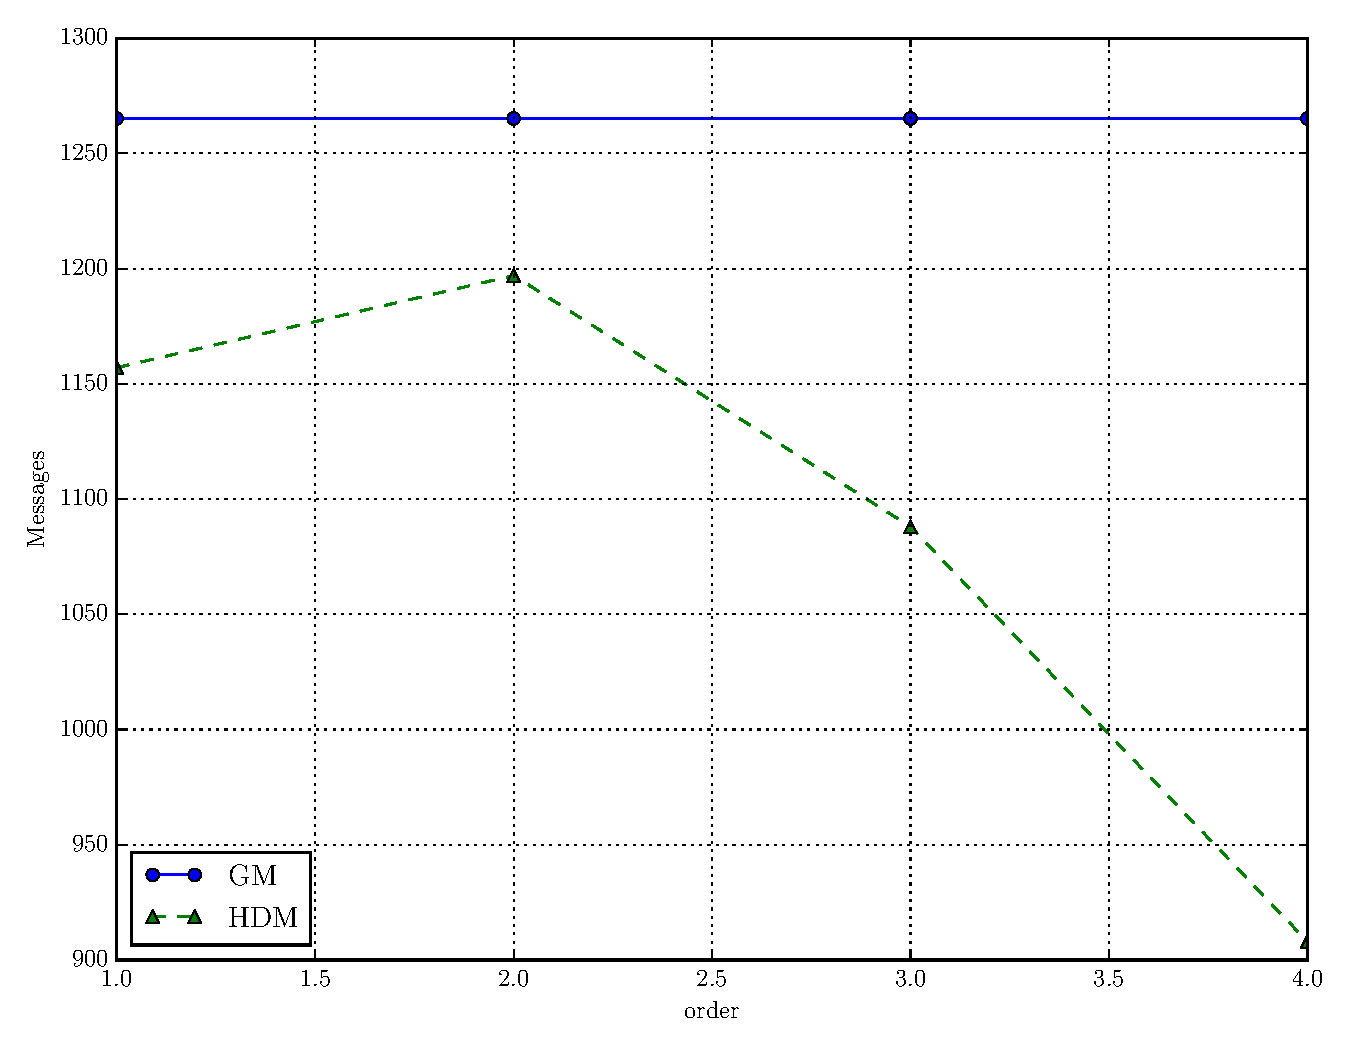
\includegraphics[width=\linewidth]{img/main_msg_interweaving_order.pdf}
  \caption{Communication cost of methods GM and HDM for the \emph{INT} dataset. The Savitzky-Golay window size is set to 40.}
\end{subfigure}\hfill
\begin{subfigure}{0.32\textwidth}%
  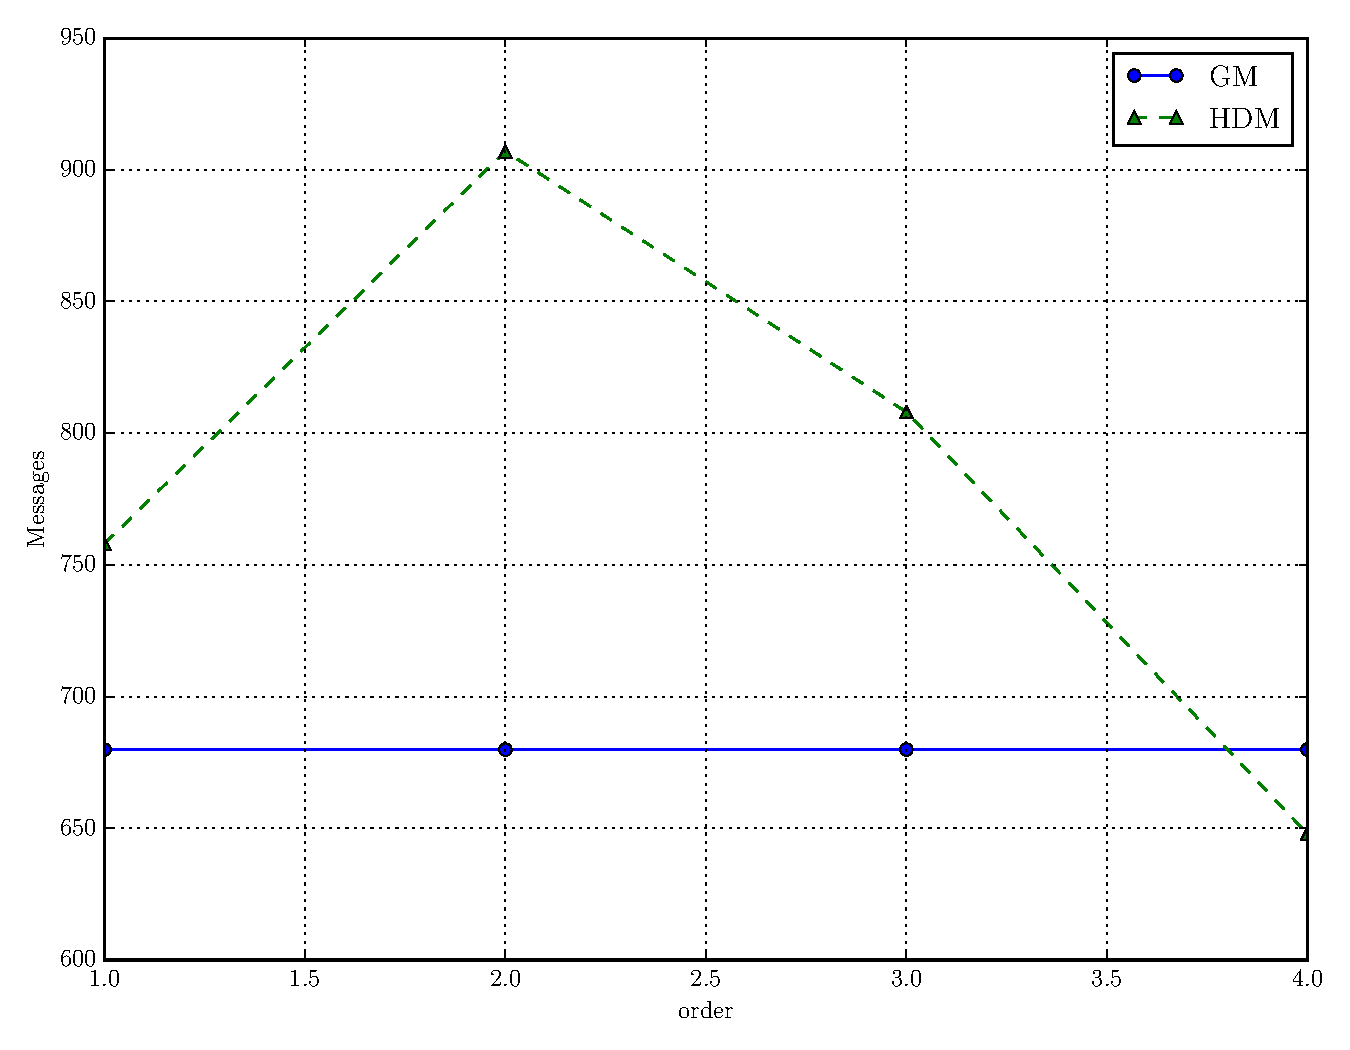
\includegraphics[width=\linewidth]{img/main_msg_noisyinterweaving_order.pdf}
  \caption{Communication cost of methods GM and HDM for the \emph{NOISE} dataset. The Savitzky-Golay window size is set to 24.}
\end{subfigure}
\vspace{0.5cm}
\caption{Comparison of the GM and HDM methods in terms of communication cost over a range of Savitzky-Golay appriximation orders, for 16 nodes.} \label{fig:mainComp-order}
\end{figure}
%%%%%%%%%%%%%%%%%%%%%%%%%%%%%%%%%%%%%%%%%%%%%%%%%%%%%%%%%%%%%%%%%%%%%%%%%%%%%%%%%%%%%%%%%%%
%%%%%%%%%%%%%%%%%%%%%%%%%%%%%%%%dims main  figure %%%%%%%%%%%%%%%%%%%%%%%%%%%%
\begin{figure}[!h]
\begin{subfigure}{0.32\textwidth}
  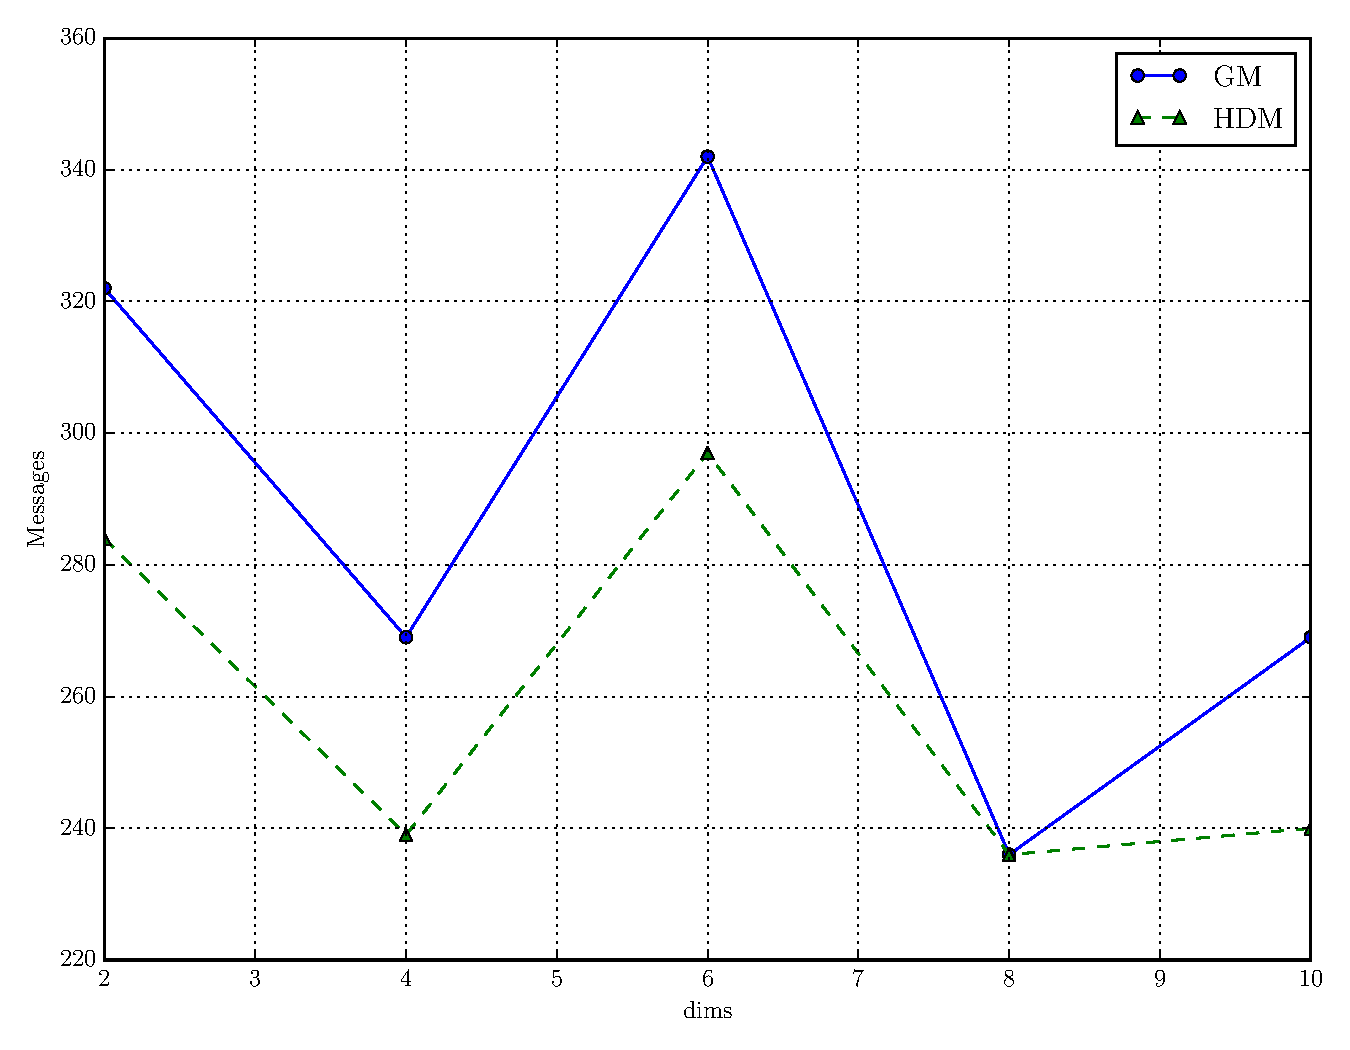
\includegraphics[width=\linewidth]{img/main_msg_linear_dims.pdf}
  \caption{Communication cost of methods GM and HDM for the \emph{LIN} dataset.}
\end{subfigure}\hfill
\begin{subfigure}{0.32\textwidth}
  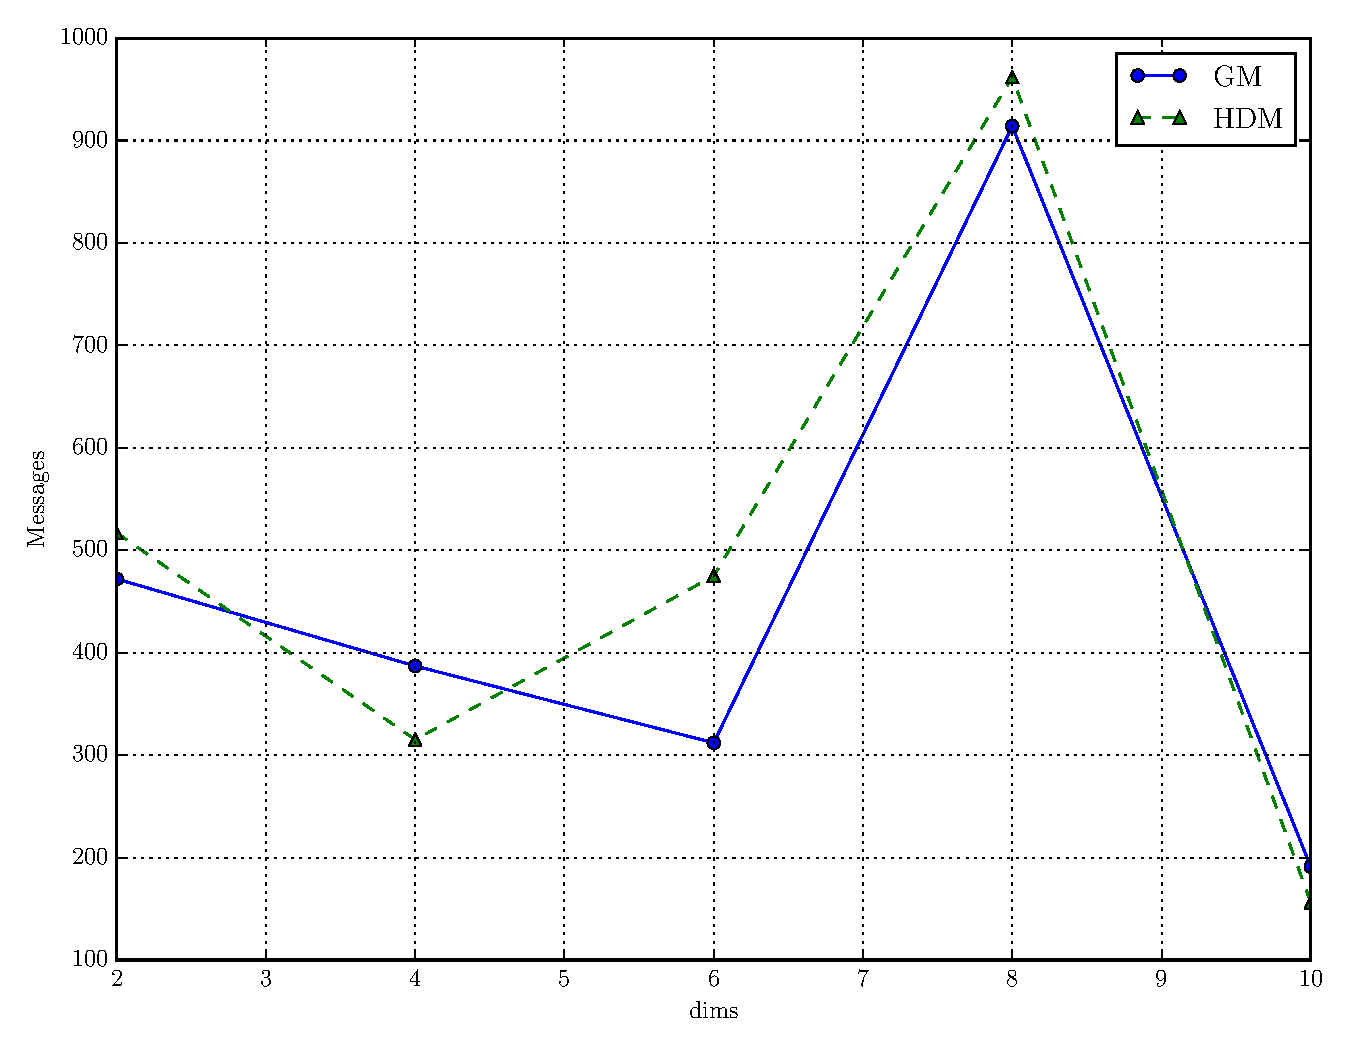
\includegraphics[width=\linewidth]{img/main_msg_interweaving_dims.pdf}
  \caption{Communication cost of methods GM and HDM for the \emph{INT} dataset.}
\end{subfigure}\hfill
\begin{subfigure}{0.32\textwidth}%
  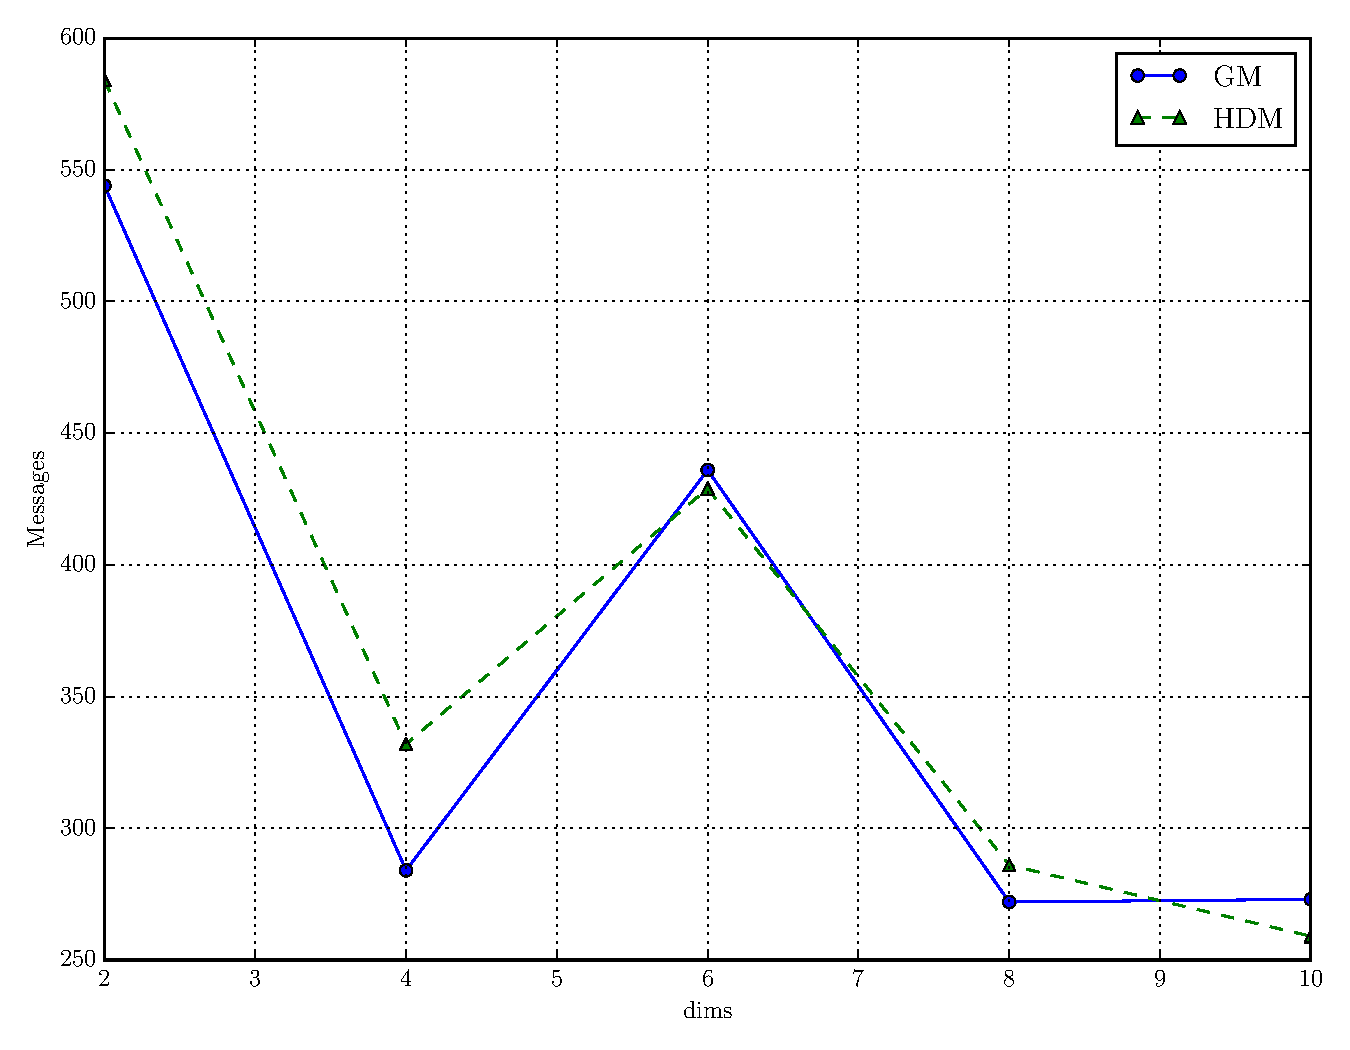
\includegraphics[width=\linewidth]{img/main_msg_noisyinterweaving_dims.pdf}
  \caption{Communication cost of methods GM and HDM for the \emph{NOISE} dataset.}
\end{subfigure}
\vspace{0.5cm}
\caption{Comparison of the GM and HDM methods in terms of communication cost over a range of stream dimensions, for 8 nodes. Savitzky-Golay's window size is set to 10 and the approximation order is set to 1 for all experiments. The monitoring function is a multi-variable quadratic function dependent on the stream dimensionality.} \label{fig:mainComp-dims}
\end{figure}
%%%%%%%%%%%%%%%%%%%%%%%%%%%%%%%%%%%%%%%%%%%%%%%%%%%%%%%%%%%%%%%%%%%%%%%%%%%%%%%%%%%%%%%%%%%


%%%%%%%%%%%%%%%%%%%%%%%%%%%%%%%%drifts main lin figure %%%%%%%%%%%%%%%%%%%%%%%%%%%%
\begin{figure}[!h]
\begin{subfigure}{0.49\textwidth}
  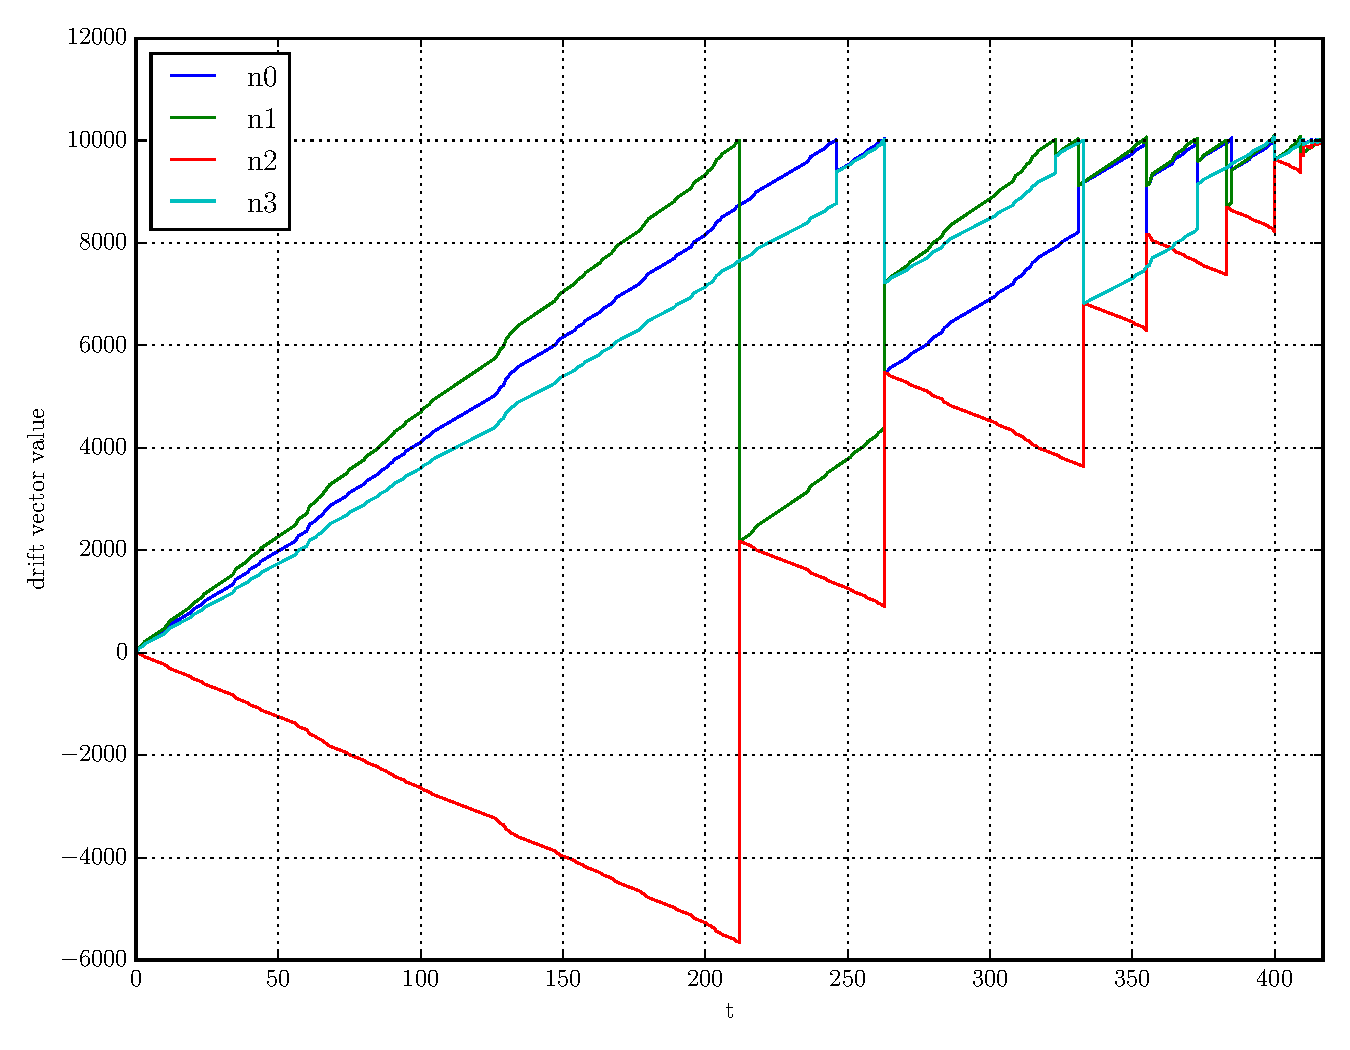
\includegraphics[width=\linewidth]{img/main_classic_drifts_linear4N.pdf}
  \caption{Drift vectors of 2 nodes, as formulated by the GM algorithm.}
\end{subfigure}\hfill
\begin{subfigure}{0.49\textwidth}
  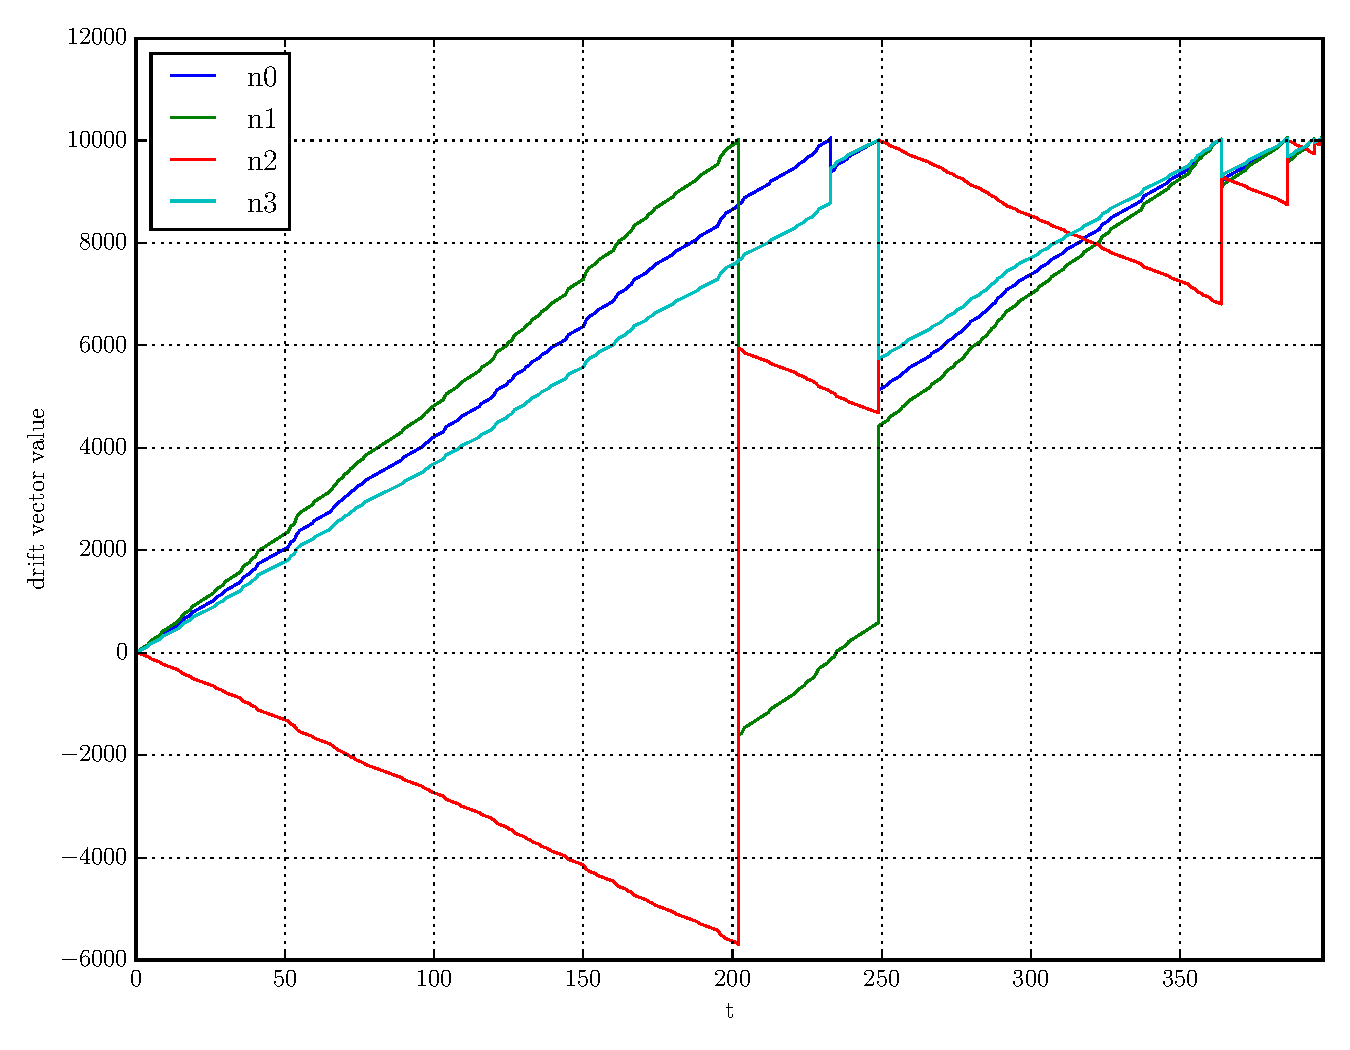
\includegraphics[width=\linewidth]{img/main_heuristic_drifts_linear4N.pdf}
  \caption{Drift vectors of 2 nodes, as formulated by the HDM algorithm.}
\end{subfigure}\hfill
\vspace{0.5cm}
\caption{The drift vectors of 2 nodes with streams originating from the \emph{LIN} dataset, when the GM and HDM methods are applied.} \label{fig:mainComp-drifts}
\end{figure}
%%%%%%%%%%%%%%%%%%%%%%%%%%%%%%%%%%%%%%%%%%%%%%%%%%%%%%%%%%%%%%%%%%%%%%%%%%%%%%%%%%%%%%%%%%%

%TODO:actual data?
\subsection{Monitoring Air Quality Data} \label{subsec:actualComp}

In this final experiment a real-world dataset is employed, originating from air quality measurements. Specifically, the variance of $NO_2$ and the ratio of $NO$ to $NO_2$ are monitored in order to evaluate the HDM and GM methods over real-world applications, once again in terms of communication costs over a range of 4 to 16 nodes, as shown in Figure~\ref{fig:actualComp}.

The HDM method exhibits a decent performance when the appropriate Savitzky-Golay parameters are carefully selected, even though the streams are characterized by great variance and irregularities in time. Compared to the GM method, the HDM method succeeds at reducing the communication overhead by approximately 10 percent.

%%%%%%%%%%%%%%%%%%%%%%%%%%%%%%%%msgs actual figure %%%%%%%%%%%%%%%%%%%%%%%%%%%%
\begin{figure}[!h]
\begin{subfigure}{0.49\textwidth}
  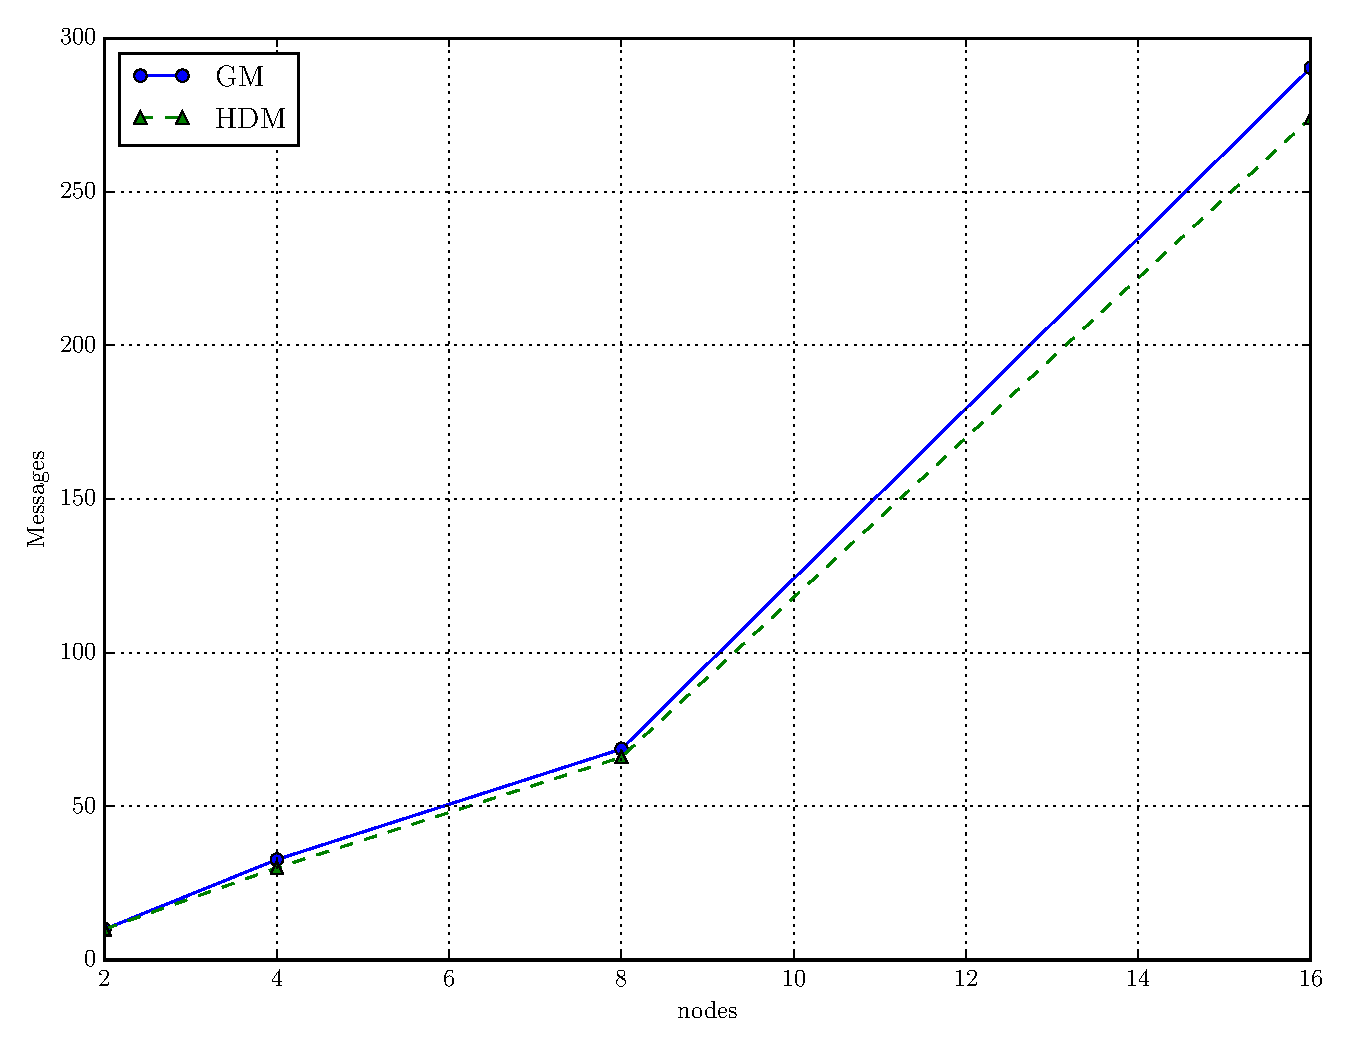
\includegraphics[width=\linewidth]{img/actual_msg_NO2_sq_2014_nodes_wl_6_order_2.pdf}
  \caption{Communication costs of methods GM and HDM over a range of 4 to 16 nodes, when variance monitoring of $NO_2$ is taking place. The Savitzky-Golay window size is set to 6 and the approximation order is set to 2.}
\end{subfigure}\hfill
\begin{subfigure}{0.49\textwidth}
  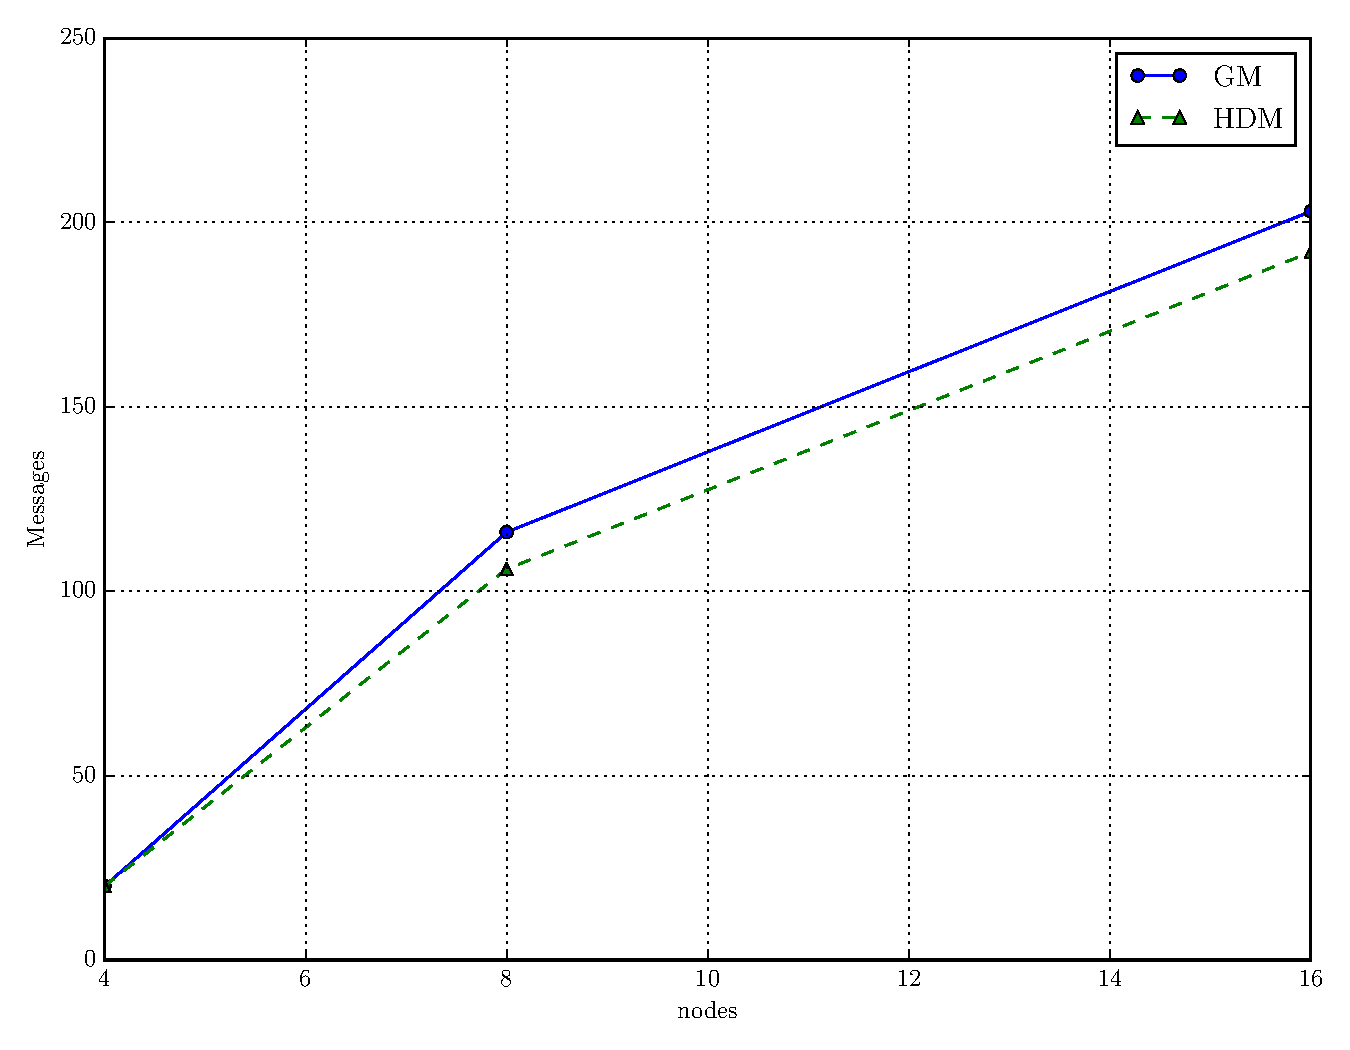
\includegraphics[width=\linewidth]{img/actual_msg_NO2_NO_2014_nodes.pdf}
  \caption{Communication costs of methods GM and HDM over a range of 4 to 16 nodes, when monitoring the ratio $NO$ to $NO_2$. The Savitzky-Golay window size is set to 10 and the approximation order is set to 1.}
  \vspace{1.2em}
\end{subfigure}\hfill
\vspace{0.5cm}
\caption{Comparison of HDM and GM methods in terms of communication cost over a range of 4 to 16 nodes originating from the air pollution dataset.} \label{fig:actualComp}
\end{figure}
%%%%%%%%%%%%%%%%%%%%%%%%%%%%%%%%%%%%%%%%%%%%%%%%%%%%%%%%%%%%%%%%%%%%%%%%%%%%%%%%%%%%%%%%%%%

